

\documentclass[default]{svmult}

% choose options for [] as required from the list
% in the Reference Guide

\usepackage{mathptmx}       % selects Times Roman as basic font
\usepackage{helvet}         % selects Helvetica as sans-serif font
\usepackage{courier}        % selects Courier as typewriter font
\usepackage{type1cm}        % activate if the above 3 fonts are
                            % not available on your system
%
\usepackage{makeidx}         % allows index generation
\usepackage{graphicx}        % standard LaTeX graphics tool
                             % when including figure files
\usepackage{multicol}        % used for the two-column index
\usepackage[bottom]{footmisc}% places footnotes at page bottom
\usepackage{times}

\usepackage{amsmath}%
\usepackage{amsfonts}%
\usepackage{amssymb}%
\usepackage{color}
\usepackage{graphicx,psfrag}
\usepackage{float}


% see the list of further useful packages
% in the Reference Guide

\makeindex             % used for the subject index
                       % please use the style svind.ist with
                       % your makeindex program

%%%%%%%%%%%%%%%%%%%%%%%%%%%%%%%%%%%%%%%%%%%%%%%%%%%%%%%%%%%%%%%%%%%%%%%%%%%%%%%%%%%%%%%%%

\begin{document}

\title*{Robust Smith Predictor Design for Time-Delayed Systems with ${H_{\infty}}$ Performance}
% Use \titlerunning{Short Title} for an abbreviated version of
% your contribution title if the original one is too long
\author{Vinicius de Oliveira, Achille Nicoletti, Alireza Karimi}
% Use \authorrunning{Short Title} for an abbreviated version of
% your contribution title if the original one is too long
\institute{Vinicius de Oliveira \at Department of Chemical Engineering, Norwegian University of Science and Technology, Norway.
\and Achille Nicoletti \at Automatic Control Laboratory, Ecole Polytechnique F\'ed\'erale de Lausanne (EPFL), Switzerland. \email{achille.nicoletti@epfl.ch}
\and Alireza Karimi (Corresponding author) \at Automatic Control Laboratory, Ecole Polytechnique F\'ed\'erale de Lausanne (EPFL), Switzerland. \email{alireza.karimi@epfl.ch}}
%
% Use the package "url.sty" to avoid
% problems with special characters
% used in your e-mail or web address
%
\maketitle

\abstract*{A new method for robust fixed-order $H_{\infty}$ controller design for uncertain time-delay systems is presented. It is shown that the $H_{\infty}$ robust performance condition can be represented by a set of convex constraints with respect to the parameters of a linearly parameterized primary controller in the Smith predictor structure. Therefore, the parameters of the primary controller can be obtained by convex optimization. The proposed method can be applied to stable single-input-single-output (SISO) and multiple-input-multiple-output (MIMO) models with uncertain dead-time and with multimodel and frequency-dependent uncertainty. It is also shown that how the design method can be extended to unstable SISO models. The design of robust gain-scheduled dead-time compensators is also investigated. The performance of the method is illustrated for both SISO and MIMO systems by simulation examples.}

\abstract{A new method for robust fixed-order $H_{\infty}$ controller design for uncertain time-delay systems is presented. It is shown that the $H_{\infty}$ robust performance condition can be represented by a set of convex constraints with respect to the parameters of a linearly parameterized primary controller in the Smith predictor structure. Therefore, the parameters of the primary controller can be obtained by convex optimization. The proposed method can be applied to stable SISO and MIMO models with uncertain dead-time and with multimodel and frequency-dependent uncertainty. It is also shown that how the design method can be extended to unstable SISO models. The design of robust gain-scheduled dead-time compensators is also investigated. The performance of the method is illustrated for both SISO and MIMO systems by simulation examples.}

\section{Introduction}
\label{sec:1}
Most industrial processes present dead time in their dynamics. Generally, dead times are caused by the time needed to transport energy, mass or information, but they also can be caused by processing time or by accumulation of time lags in a sequence of simple dynamic systems interconnected in series (\cite{NC07}).

The presence of dead times in the control loops has two main consequences: it greatly complicates the analysis and the design of feedback controllers  and it makes satisfactory control performance more difficult to achieve (\cite{Pal96}). Dead-time compensators can be used to improve the closed-loop performance of classical controllers (PI or PID controllers) for processes with delay. The Smith Predictor (SP) (See Fig.\ref{fig:dtc}), proposed in the late 1950s by \cite{Smi57}, was the first dead-time compensation structure used to improve the performance of the classical
controllers and became the most known and used algorithm to compensate dead time in the industry.

Although the SP offers potential improvement of the closed-loop performance of process with large dead-time, it requires a good model since small modeling errors can lead to very poor performance. %In fact, even if the SP is nominally stabilizing, the closed-loop system may become unstable for infinitesimal change in the process dynamics (\cite{Pal80}).
For this reason, research efforts have been focused on robustness issues of the SP. A tuning method for models with one uncertain parameter is proposed by \cite{Bro79}.
Easy tuning rules for SP in the presence of dead-time uncertainty is addressed in \cite{SS93} and a guideline for selection the closed-loop bandwidth based on the dead-time uncertainty bound is proposed.
In \cite{PB94}, a robust tuning rule is developed  which considers the modeling error in the dead time.  Robust PID tuning for SP considering model uncertainty is proposed by \cite{LLSL99}. In particular, first and second order plus dead-time systems which may contain uncertainty in multiple parameters of the model are considered. In \cite{MZ00}, tuning guidelines are presented for setpoint tracking considering model mismatches in the dead-time. 

Many researchers are interested in the optimal control of dead-time
systems, especially $H_{\infty}$ control, i.e., to find a controller to
internally stabilize the system and to minimize the $H_{\infty}$-norm of an associated transfer
function. Many relevant results have been presented in this framework using 
modified versions of the SP. See, for instance, \cite{Mir03}, \cite{MZ00} and \cite{Zho03a}. Recently, the SISO SP has been extended and generalized for MIMO systems. In \cite{SBP09}, a structured uncertainty approach was implemented for SP's with diagonal delay matrices. This method, however, does not consider general and distinct time delays for each element of the plant transfer matrix. A diagonal $H_2$ optimal controller for non-square plants is designed by factorization methods in \cite{ZL06}. In \cite{NC00}, a generalized predictive control (GPC) method is implemented on MIMO SP systems with multiple delays.  
Nonetheless, these control techniques are quite complex and their implementation can be involved.


%Nonetheless, as pointed out by \cite{Zho03b}, these controllers are too involved and the predictor always includes additional unstable hidden modes even for stable plants. As the author argues, these hidden modes are not safe as they tend to destabilize the system when implemented. Therefore, the practical significance of these results are limited.

This paper presents a new method to design fixed-order SP controllers that considers uncertainty simultaneously in the dead-time and in the rational part of the model.  The performance specification, like the standard $H_{\infty}$ control problem, is a constraint on the infinity norm of the weighted sensitivity function and is represented by a set of convex constraints in the Nyquist diagram. The extension to MIMO systems will be based on the idea presented in \cite{GKL10b} for designing decoupling MIMO controllers. In \cite{GKL10b}, a convex optimization approach was implemented to design a linearly parameterized controller for a MIMO system. In this paper, this concept will be extended to MIMO SP's with process plants that possess uncertain time delays. 
%A line search on the upper bound $\gamma$ of the infinity norm of the weighted sensitivity function can be used in association to a convex feasibility problem to determine the primary controller parameters. The proposed method can be used for PID primary controllers, which are of great practical interest, as well as for higher order linearly parametrized controllers in discrete or continuous time.

%It is important to point out that a method to design fixed-order controllers for standard control loops based on convex constraints in the Nyquist diagram has been firstly proposed in \cite{KG10}. Although, this method can be used for time-delay systems, it does not explore the structure of Smith Predictor to compensate for time delay. This may lead to very high order controller or poor performance. This paper uses the same framework to design Smith Predictor compensators for time-delay systems. 

This paper is organized as follows: In Section \ref{sec:2} the class of models, controllers and the control objectives for SISO systems are
defined. Section \ref{sec:3} will extend the class of controllers and control objectives to MIMO systems. Sections \ref{sec:2} and \ref{sec:3} will also discuss the control design methodology and stability conditions for the SISO and MIMO Smith predictor configurations, respectively. This methodology is based on the convex constraints in the Nyquist diagram. In Section \ref{sec:4} the results are extended to unstable time-delay SISO systems. Gain-scheduled SP is designed for time-delay systems in Section \ref{sec:5}. Each section will end with an illustrative example. Finally the concluding remarks are given. 


\section{SISO Problem Formulation}
\label{sec:2}
\subsection{Class of models}
Consider the class of stable time-delay LTI-SISO systems with bounded infinity norm. It is assumed that the plant model can be represented by:
\begin{equation}\label{model}
P(s)=G(s)e^{-\tau s}
\end{equation}
where the time delay $\tau$  is unknown but belongs to a finite set $\{\tau_1, \tau_2, \ldots, \tau_q \}$ and the dead-time free part of the model has unstructured multiplicative uncertainty described as:
\begin{equation}\label{uncertainty}
G(s)=G_n(s)[1+\Delta(s) W_2(s)]
\end{equation}
where $W_2(s)$ is a known stable uncertainty filter, $G_n(s)$ the nominal dead-time free model and  $\Delta(s)$  an unknown stable transfer function with $\| \Delta\|_{\infty}<1$.  
Therefore, we can assume that $P(s)$ belongs to a set $\mathbb{P}$ of $q$ models given by:
\begin{equation}
\mathbb{P}\stackrel{\triangle}{=}\{ P_i(s)[1+\Delta(s) W_2(s)]; \: i=1,\dots, q \}
\label{setP}
\end{equation}
where $P_i(s)=G_n(s)e^{-\tau_i s}$.
%We can also define the set of nominal models as:
%\begin{equation}
%\mathcal{P}_n\stackrel{\triangle}{=}\{ P_i(s)=G_n(s)e^{-\tau_i s}; \: i=1,\dots, q \}
%\label{setPn}
%\end{equation} 

\subsection{Class of controllers} \label{sec:siso_cls}

The SP control structure shown in Fig.\ref{fig:dtc} is considered. The nominal model $P_0(s)=G_n(s)e^{-\tau_n s}$ with $\tau_n \in [\tau_1, \tau_q ]$ is used for the implementation of the controller.
\begin{figure}[h]
\centering
\psfrag{rr}{\small $r$}
\psfrag{cc}{\small $C(s)$}
\psfrag{uu}{\small $u$}
\psfrag{pp}{\small $P(s)$}
\psfrag{gn}{\small $G_n(s)$}
\psfrag{ex}{\small $e^{-\tau_n s}$}
\psfrag{yp}{\small $y_p$}
\psfrag{yy}{\small $y$}
\psfrag{pl}{\small $+$}
\psfrag{mi}{\small $-$}
\psfrag{dis}{\small $d$}
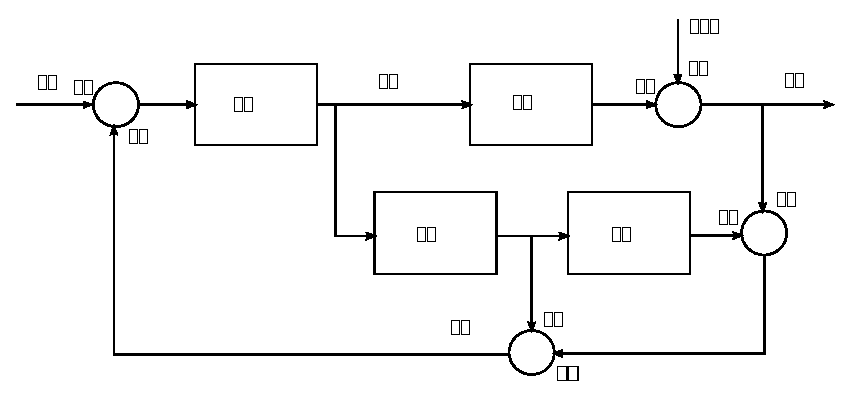
\includegraphics[width=0.8\columnwidth]{fig/SISO_block.eps}
\caption{Smith Predictor}
\label{fig:dtc}
\end{figure}%

The primary controller $C(s)$ is linearly parametrized by
\begin{equation}\label{eq:controller}
C(s)= \rho^T \phi(s)
\end{equation}
 where 
$
 \rho^T=[\rho_1,\rho_2, \ldots, \rho_{n_c}] 
$
is an $n_c$ dimensional vector of the controller parameters and $\phi^T(s)=[\phi_1(s),\phi_2(s), \ldots, \phi_{n_c}(s)]$ is a vector of basis functions with $\phi_i(s)$ transfer functions with no RHP poles. For instance, a PID controller could be linearly parametrized by
$$\rho^T=[K_p,K_i, K_d] \quad , \quad  \phi^T(s)=[1, \frac{1}{s},\frac{s}{1+T_fs}] $$

\subsection{Design specifications}

As stated in \cite{DFT92}, the sensitivity and complementary functions of a system are invoked to test the robust performance and robust stability conditions. From Fig. \ref{fig:dtc}, the sensitivity functions for the nominal models $P_i(s)$ can be determined by obtaining the transfer function from the output disturbance $d$ to the system output $y$:
\begin{equation}\label{eq:sensitivity}
S_i(s)=\frac{1+C(s)H(s)}{1+C(s)[H(s)+P_i(s)]}
\end{equation}
where $H(s)=G_n(s)-P_0(s)=G_n(s)(1-e^{-\tau_n s})$. The complementary sensitivity functions for the nominal models will be the transfer function from the reference input $r$ to $y$ (which is also equal to $1-S_i(s)$):
\begin{equation}\label{eq:sensitivity_comple}
T_i(s)=\frac{C(s)P_i(s)}{1+C(s)[H(s)+P_i(s)]}
\end{equation}
A standard robust control problem is to design a controller that satisfies $\| W_1S_i\|_{\infty}<1$ for a set of models where $W_1(s)$ is the performance weighting filter. If the model is described by unstructured multiplicative uncertainty, the necessary and sufficient condition for robust performance is given by \cite{DFT92}:
\begin{equation}\label{eq:robust_performance}
\|  |W_1S_i| + |W_2T_i| \|_{\infty}<1  \quad \mbox{for} \quad i=1,\ldots, q
\end{equation}
The goal of the proposed approach is to design the primary controller $C(s)$ in the SP structure to guarantee robust performance of the closed-loop system. 

\subsection{Proposed method} \label{sec:siso_pro}

The robust performance condition (\ref{eq:robust_performance}) can be written as: 
\begin{equation}\label{eq:robust_performance2}
\left| W_{1}(j\omega)S_i(j\omega)| + |W_{2}(j\omega)T_i(j\omega) \right|<1,\quad \forall \omega
\end{equation}
for $i=1,\ldots, q$. Let $L_i(s,\rho)$ be defined as the open-loop transfer function of the SISO SP. From Fig. \ref{fig:dtc}, the transfer function from the input of $C(s)$ to $y_p$ will represent this open-loop transfer function:
\begin{equation}
L_i(s,\rho)=C(s,\rho)(H(s)+P_i(s))
\end{equation} 
The dependency on frequency $\omega$ and $s$ will be omitted for brevity but the dependency on the controller parameter $\rho$ will be highlighted. 

The main result of this section is given in the following theorem.
\begin{theorem}\label{th:siso}
Consider the  set of models $\mathbb{P}$  in (\ref{setP}) with multiplicative uncertainty filter $W_{2}(j\omega)$, then the linearly parametrized controller in (\ref{eq:controller}) in the SP structure guarantees closed-loop stability and satisfy the following robust performance condition:
\begin{equation} \label{RobPer}
\| |W_{1}S_i| + |W_{2}T_i|  \|_{\infty}<1\quad \mbox{for }i=1,\ldots,q  
\end{equation}
if
\begin{multline} \label{eq:cond_theorem1}
\left[\big|W_{1}(j\omega)[1+C(j\omega,\rho)H(j\omega)] \big | \right.+ 
\left.\big | W_{2}(j\omega)C(j\omega,\rho)P_i(j\omega) \big | \right] |1+L_d(j\omega)|  \\
- Re\{[1+L^{\ast}_d(j\omega)][1+L_i(j\omega,\rho)]\}<0 \\  \forall \omega \quad \mbox{ for }i=1,\ldots,q
\end{multline}
where $L_d(j\omega)$ is a strictly proper transfer function which does not encircle the critical point and $L_d^*(j\omega)$ is its complex conjugate. 
\end{theorem}

\begin{proof} 
\smartqed
Since the real part of a complex number is less than or equal to its magnitude, we have
\begin{equation} \label{UpperBound}
Re\{[1+L^{\ast}_d][1+L_{i}(\rho)]\}\leq |[1+L^{\ast}_d][1+L_{i}(\rho)]|
\end{equation}
Then, using (\ref{eq:cond_theorem1}) and the fact that $|1+L_d|=|1+L^*_d|$, one obtains 				
\begin{eqnarray}
\big|W_{1}(1+C(\rho)H)\big| + \big | W_{2}C(\rho)P_i \big| - 
|1+L_i(\rho)|<0 \nonumber\\
 \forall \omega \: \mbox{ for }i=1,\ldots,q 
\end{eqnarray}
Using $L_i(\rho)=C(\rho)(H+P_i)$ we have 
\begin{eqnarray}\label{eq:siso_rob}
\frac{|W_{1}(1+C(\rho)H)| + |W_{2}C(\rho)P_i | }{|1+C(\rho)(H+P_i)|} <1 \nonumber\\
 \forall \omega \: \mbox{ for }i=1,\ldots,q  
\end{eqnarray}
that leads directly to (\ref{RobPer}).
To prove that all  closed-loop transfer functions are stable, consider (\ref{eq:cond_theorem1})  which gives:
\begin{equation}
Re\{[1+L^{\ast}_d(j\omega)][1+L_i(j\omega,\rho)]\}>0 \quad \forall \omega
\end{equation}
or, alternatively, 
\begin{equation}
wno\{[1+L^{\ast}_d(j\omega)][1+L_i(j\omega,\rho)] \}=0
\end{equation}
where $wno$ stands for winding number around the origin. Since both $L^{\ast}_d(j\omega)$ and $L_i(j\omega,\rho)$ are constant or zero for the semi-circle with infinity radius of the Nyquist contour 
the $wno$ depends only on the variation of $s$ in the imaginary axis. Thus,
\begin{equation}
wno\{[1+L_d(j\omega)]\}  =wno\{[1+L_i(j\omega,\rho)] \}
\end{equation}
Since $L_d(j\omega)$ satisfies the Nyquist stability criterion $L_i(j\omega,\rho)$ will do so and 
all zeros of $1+L_i(j\omega,\rho)$ will be in the left-hand side of the complex plan. Since the zeros of
$1+L_i(j\omega,\rho)$ are the closed-loop poles, the system will be internally stable.
\qed
\end{proof}


\subsection{Primary controller design}
The problem of minimizing the upper bound $\gamma$ of the infinity norm of the weighted sensitivity function is considered. Therefore, the primary controller should be obtained from the following optimization problem: 
\begin{eqnarray}\label{eq:min_hinf}
\min_{\rho} \gamma \nonumber \\\mbox{Subject to:}\\ \nonumber
 \|  |W_1S_i| +& |W_2T_i| \|_{\infty}<\gamma \quad \mbox{for } i=1,\dots,q\nonumber
\end{eqnarray}
This optimization can be convexified using Theorem \ref{th:siso} and solved by an iterative bisection algorithm. At each iteration $j$, $\gamma_j$ is fixed and $W_1$ and $W_2$ are replaced by $W_1/\gamma_j$ and $W_2/\gamma_j$. Then, a feasibility problem is solved under the convex constraints (\ref{eq:cond_theorem1}). If the problem is feasible, $\gamma_{j+1}$ is chosen smaller than $\gamma_{j}$. Otherwise $\gamma_{j+1}$ is increased.

Notice that the condition (\ref{eq:cond_theorem1}) is defined for every frequency $\omega$ leading to infinite number of constraints. In practice, a frequency  grid can be used  with a sufficiently large number of frequency points $N$ (a finer grid can be used around the crossover frequency). The effect of gridding on the stability and performance of the closed loop system has been studied in \cite{GKL10a}.

{\bf Remark I:} 
The constraint in (\ref{eq:cond_theorem1}) is an inner convex approximation of the non convex constraint in (\ref{RobPer}) or 
(\ref{eq:robust_performance2}). The quality of this approximation depends on the choice of $L_d$.  It can be shown that better approximation is achieved if $L_d$ is chosen such that its frequency response is close to that of $L_i(\rho)$ (\cite{KG10}). 

%Note that $L_i(\rho)$ can be written as:
%\begin{equation}\label{eq:new_ld}
%L_i(\rho)=C(\rho)G_n+C(\rho)(P_i-P_0)\end{equation}Therefore, If  $\tau_i$ is close to $\tau_n$ or the model mismatch $P_i-P_0$ is small, $L_{d}$ can be seen as the desired open loop transfer function of the system without dead-time, i.e.,  $C(\rho)G_n$.  For systems with large uncertainty in the time delay, different $L_d$ can be considered for each model $P_i$. Since it is desired to obtain an open-loop transfer function which is ideally $C(\rho)G_n$, we can substitute $C(\rho)\approx L_d/G_n$ in (\ref{eq:new_ld}). In this case, $L_{d_i}$ can be computed as follows:\begin{equation}{L}_{d_i}=L_{d}+\frac{L_d}{G_n}(P_i-P_0)\end{equation}To ensure stability, for stable plant models, the number of counterclockwise encirclements of $L_d$ around the critical point should be equal to zero. An iterative algorithm can be used to improve the results. In  this algorithm $L_d$ in the $(k+1)$-th iteration is computed using the controller of the last iteration  $C_{k}(\rho)$ and (\ref{eq:new_ld}):\begin{equation}{L}_{d_i}=C_{k}(\rho)G_n+C_k(\rho)(P_i-P_0)\end{equation}

%\textbf{Remark II:}
%It is also possible to handle multimodel uncertainty in the proposed approach. Consider that the plant  belongs to a set of stable models $\mathcal{P}$ where:
%\begin{equation}
%\mathcal{P} = \{ G_1e^{-\tau_1 s}, G_2e^{-\tau_2 s},\ldots, G_me^{-\tau_m s}  \}
%\end{equation}
%It is assumed that nominal model $P_0=G_ne^{-\tau_n s}$ representing the set is available. In this case, the robust performance condition is
%\begin{equation}
% \|  W_{1i}S_i \|_{\infty}<\gamma \quad \mbox{for } i=1,\dots,m
%\end{equation}
%which can be approximated by the following convex constraints:
%\begin{multline} \label{eq:cond_multi}
%|W_{1i}(j\omega_k)[1+C(j\omega_k,\rho)H(j\omega_k)] [1+L_{d_i}(j\omega_k)]|- \\
%Re\{[1+L^{\ast}_{d_i}(j\omega_k)][1+L_i(j\omega_k,\rho)]\}<0 \\
%k=1,\ldots,N; m=1,\ldots, m 
%\end{multline}
%Note that different performance specification can be defined for each model in the set (by different $W_{1i}$ and $L_{d_i}$). 

\subparagraph{Example 1}
Consider the process described by (\ref{model}) with multiplicative uncertainty as in (\ref{uncertainty}) with 
\begin{equation}
G_n(s)=\frac{1}{(5s+1)(10s+1)}
\end{equation}
and 
\begin{equation}
 W_2(s)=\frac{ -s^2 - 2 s}{s^2 + 2 s + 1}
\end{equation}
The unknown time delay $\tau$  belongs to the set $\{4.5, 5, 5.5\}$.
The nominal model used in the SP structure is chosen as $P_0(s)=G_n(s)e^{-5s}$.
%By griding the range of allowable dead-times a set $ \mathcal{P}=\{P_i(s),\: i=1,\ldots,q\}$ of models is generated where:
%\begin{equation}
%P_i(s)=G_n(s)e^{-\tau_is}, \; i=1,\ldots,q
%\end{equation}
%In this example $q=3$ is chosen. 
The performance specification is defined by the following filter:
 \begin{equation}
 W_1(s)=\frac{2}{(30s+1)^2}
\end{equation}
A PID primary controller with $T_f=0.01$ that minimizes $\| |W_1S_i|+|W_2T_i|  \|_{\infty}<\gamma$ for $i=1,2,3$ should be computed.

Since the controller has an integrator, $L_d$ is chosen as $L_d(s)=\omega_c/s$ where $\omega_c=0.1$ rad/s which is 20\% higher than open loop bandwidth. Then, the optimization problem (\ref{eq:min_hinf}) is solved considering $N=100$ equally spaced frequency points between $10^{-3}$ and $10^3$ rad/s. The resulting primary controller is:
\begin{equation}
C(s)=\frac{12.3 s^2 + 3.28 s + 0.2201}{0.01 s^2 + s}
\end{equation}
and leads to $\gamma=0.313$.
This controller is compared to that proposed in \cite{Kay01}. Kaya's controllers performs better than other controllers presented in the literature (\cite{PB94}, \cite{Hag92} and \cite{HWC95}).
Fig. \ref{fig:example1} depicts 
the performance of both controller on unitary step setpoint change considering the time-delay $\tau=4.5s$, $\tau=5.0s$ and $\tau=5.5s$. As it can be seen, both controller performed well, however, the proposed controller achieves faster response. % (see Table \ref{table:performance}).
\begin{figure}[H]
\centering
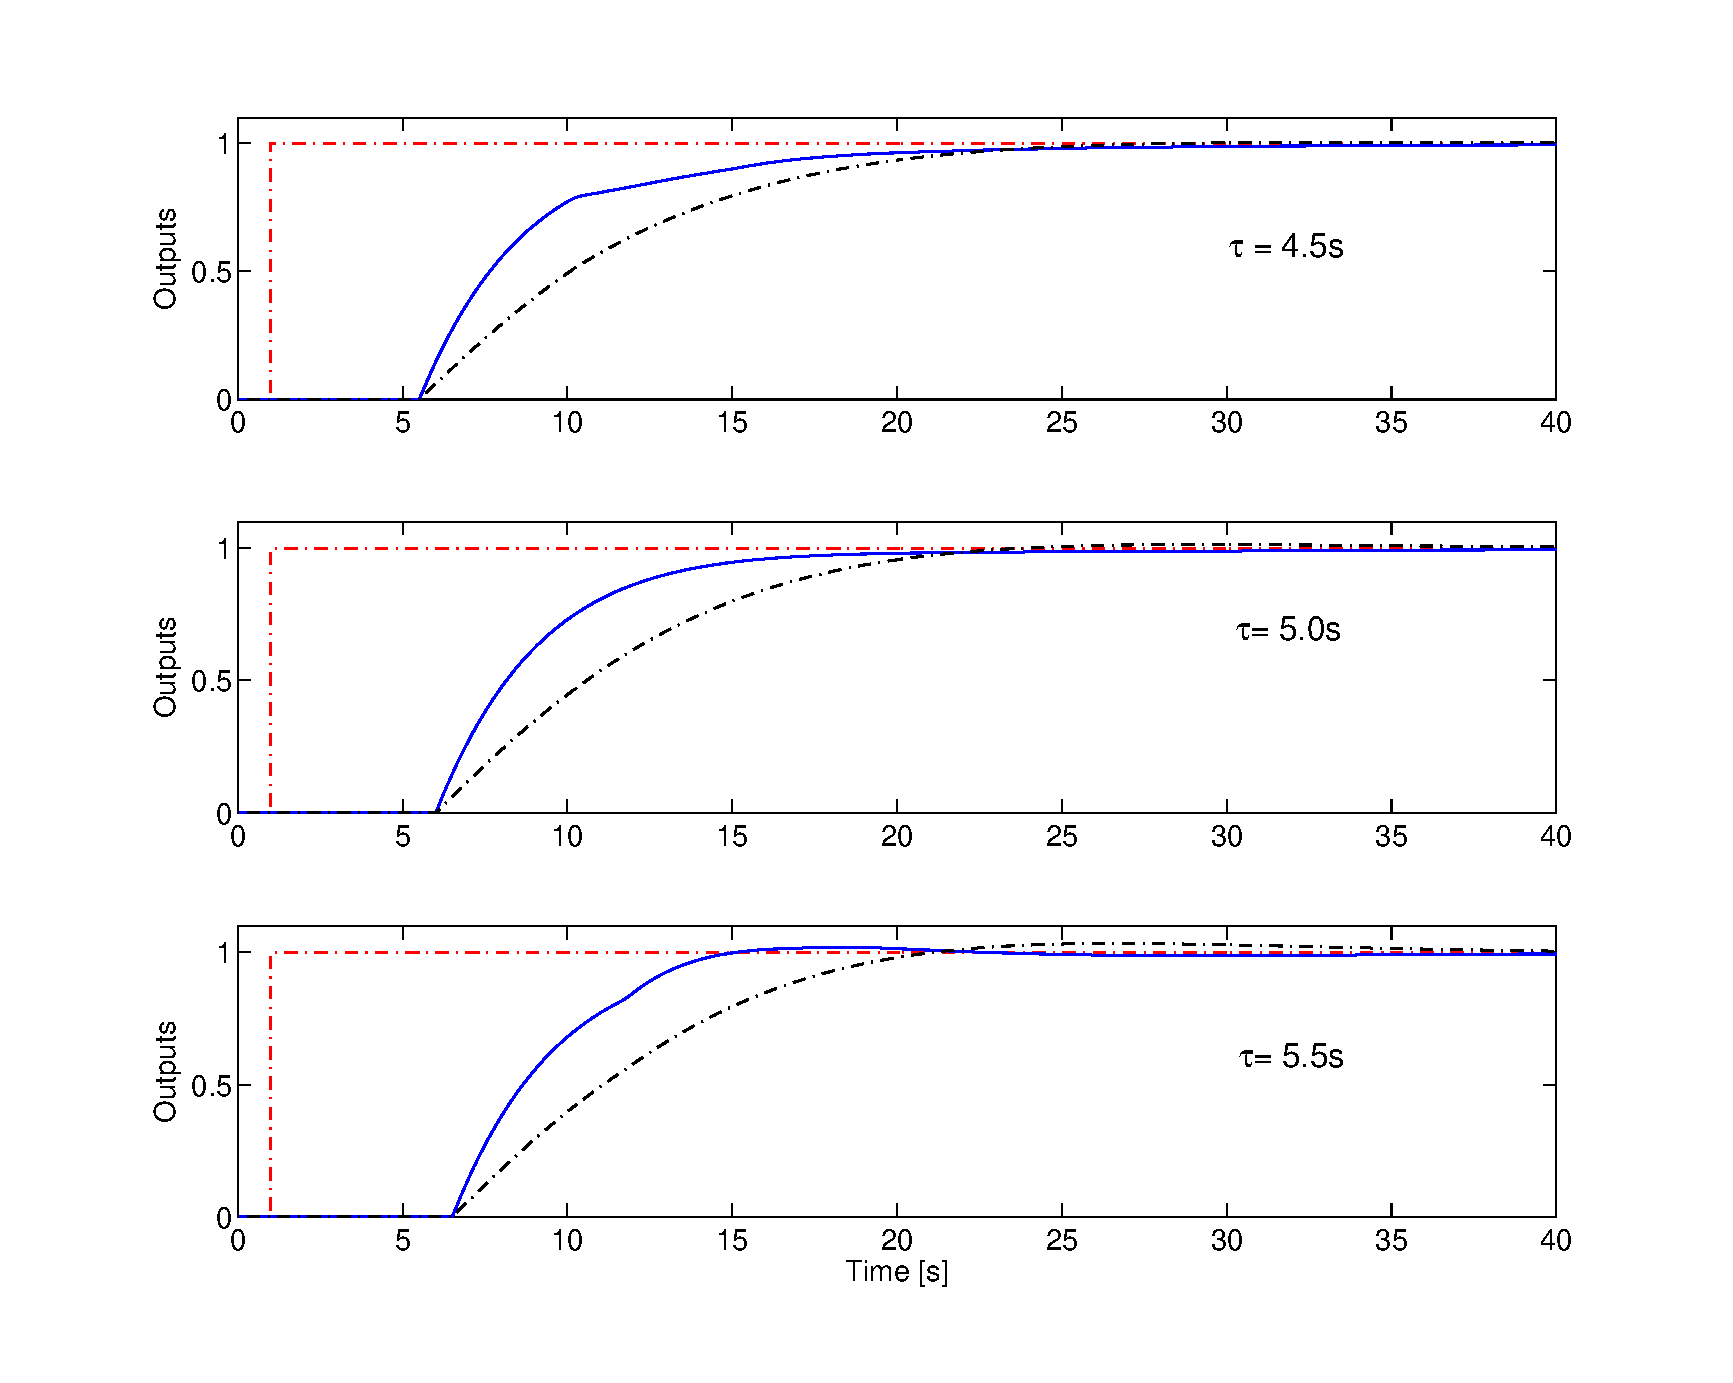
\includegraphics[scale=0.31]{fig/example1_final_paper}
\caption{Example 1: Blue solid line: proposed;  black dot-dashed line: ref \cite{Kay01} }
\label{fig:example1}
\end{figure}%
\section{MIMO Problem Formulation}
\label{sec:3}
In this section, the SP for MIMO systems with generalized time delays will be investigated . An example of how to design a linearly parameterized MIMO controller for such a system will be presented at the end of this section. For notation purposes, bold face characters will represent transfer function matrices.
\subsection{Class of models}
Let $n_o$ and $n_i$ represent the number of outputs and the number of inputs of a system, respectively. The set of all LTI-MIMO strictly proper uncertain models with uncertain time delays can be defined as follows: 
\begin{equation}\label{eq:setpmimo}
\mathcal{P}=\{\vec{P}_c(s)[\vec{I}+\Delta \vec{W}_2]; c=1,\ldots,m\}
\end{equation}
where each element in $\vec{P}_c(s)$ possesses a time delay that can vary over a range of specified values, and $\vec{W}_2$ is a matrix that represents the multiplicative input uncertainty of the system. For simplicity, one model from the set $\mathcal{P}$ will be investigated, and the subscript $c$ will be omitted. The uncertain $n_o \times n_i$ time delayed plant has the following form:
\begin{equation}\label{eq:mimo_p}
\vec{P}(s)=
\begin{bmatrix}
G_{11}(s)e^{-\tau_{11} s} & \cdots & G_{1n_{i}}(s)e^{-\tau_{1n_{i}} s} \\ \vdots & \ddots & \vdots \\ G_{n_{o}1}(s)e^{-\tau_{n_{o}1} s} & \cdots & G_{n_{o}n_{i}}(s)e^{-\tau_{n_{o}n_{i}} s}
\end{bmatrix}
\end{equation}
where $G_{qp}(s)$ is a strictly proper delay-free transfer function, and $\tau_{qp}$ is the uncertain time-delay of the process for $p=1,\ldots, n_i$ and $q=1,\ldots, n_o$. 


\subsection{Class of controllers}
As stated in \cite{GKL10b}, an $n_i \times n_o$ matrix can be formed to represent the controller $\vec{K}(s,\rho)$. The elements of $\vec{K}(s,\rho)$ will possess linearly parameterized elements $K_{pq}(s)=\rho^T_{pq}\phi_{pq}(s)$, where $\rho^T_{pq}$ is a vector of parameters, and $\phi_{pq}(s)$ is a vector of stable transfer functions chosen from a set of orthogonal basis functions. The non-diagonal elements of $\vec{K}(s,\rho)$ strive to decouple the system, while the diagonal elements aim to control the single-loop subsystems. As with the SISO case, the main purpose of parameterizing the controller in this manner is due to the fact that the components of the open loop transfer function can be written as a linear function of the control parameters $\rho$,
\begin{equation}
\rho=[\rho_{11},\ldots,\rho_{1_{n_{i}}},\ldots,\rho_{n_{o}1},\ldots,\rho_{n_{o}n_{i}}]
\end{equation}
\subsection{Design specifications}\label{sec:mimo_des}
Fig. \ref{fig:mimo_block} displays the SP for the MIMO case,
%\footnote{Note that the block diagram for the SP has been reconfigured for the MIMO case. In this manner, the uncertain plant is generalized where each element in (\ref{eq:mimo_p}) can posses a distinct and unique range of time delays.}. 
where $\vec{G}_n(s)$ is an $n_o \times n_i$ nominal delay-free transfer function matrix with elements $G_{qp}(s)$, and $\vec{P}_n(s)$ is an $n_o \times n_i$ nominal transfer function matrix which includes the nominal values of the time delays, which is comprised of elements $G_{qp}(s)e^{-\zeta_{qp}}$ (where $\zeta_{qp}$ represents the $qp$-th nominal time delay). Both $\vec{Y}(s)$ and $\vec{X}(s)$ are $n_o \times 1$ column vectors that possess elements $y_q(s)$ and $x_q(s)$, respectively. The transfer function from the inputs of $\vec{C}(s)$ to $\vec{Y}_p(s)$ will represent the open-loop transfer function,
\begin{equation}\label{eq:oltfmimo}
\vec{L}(s)=[\vec{P}(s)+\vec{H}(s)]\vec{C}(s)
\end{equation}
where $\vec{H}(s)=\vec{G}_n(s)-\vec{P}_n(s)$. Notice that if $\vec{P}(s)=\vec{P}_n(s)$, then $\vec{L}(s)=\vec{G}_n(s)\vec{C}(s)$. Since the class of controllers to be designed for this system are linearly parameterized, the elements of the controller $\vec{C}(s)$ will actually be a function of the controller parameters $\rho$. Therefore, $\vec{C}(s)$ will be represented as $\vec{C}(s,\rho)$.
\begin{figure}
\centering
\psfrag{cc}{$\vec{C}(s)$}
\psfrag{yy}{$\vec{Y}(s)$}
\psfrag{yp}{$\vec{Y}_p(s)$}
\psfrag{pp}{$\vec{P}(s)$}
\psfrag{pl}{$+$}
\psfrag{mi}{$-$}
\psfrag{gn}{$\vec{G}_n(s)$}
\psfrag{gnd}{$\vec{P}_n(s)$}
\psfrag{dd}{\hspace{-0.2cm}$\vec{D}(s)$}
\psfrag{uu}{$\vec{U}(s)$}
\psfrag{rr}{\hspace{-0.1cm} $\vec{X}(s)$}
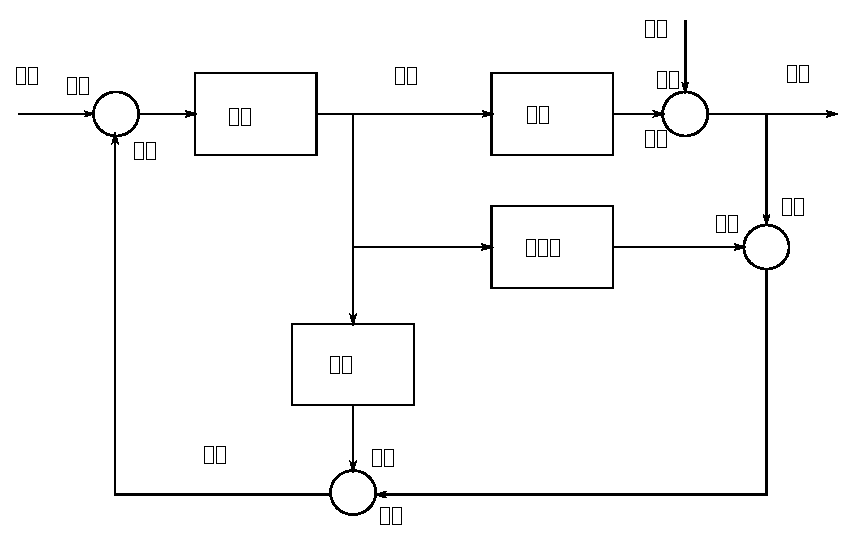
\includegraphics[scale=0.6]{fig/mimo_b3.eps}
\caption{MIMO representation of the Smith Predictor}
\label{fig:mimo_block}
\end{figure}
%For MIMO systems, the robust stability conditions are dependent on the type of perturbed model. For example, the robust conditions for MIMO systems with input multiplicative perturbations will differ for systems with output multiplicative perturbations. For a system with multiple unstructured uncertainties, the structured singular value method is typically used to prove the robust stability and robust performance of a system \cite{ZhoDoy}. 

The transfer function from the output disturbance $\vec{D}(s)$ to $\vec{Y}(s)$ is the output sensitivity function $\vec{S}(s,\rho)$, while the transfer function from $\vec{X}(s)$ to $\vec{Y}(s)$ is the complementary sensitivity function $\vec{T}(s,\rho)$:
\begin{align}\label{eq:sens_mimo}
&\vec{S}(s,\rho)=[\vec{I}+\vec{H}(s)\vec{C}(s,\rho)]\vec{Z}^{-1}(s,\rho) \nonumber\\ &\vec{T}(s,\rho)=\vec{P}(s) \vec{C}(s,\rho) \vec{Z}^{-1}(s,\rho)
\end{align}
where $\vec{Z}(s,\rho)=[\vec{I}+\vec{L}(s,\rho)]$. As with the SISO case, the goal here is to determine the controller $\vec{C}(s,\rho)$ that will guarantee the robust performance and robust stability of the closed-loop SP system. 

%Note that $\vec{S}(s,\rho)$ and $\vec{T}(s,\rho)$ will in general contain non diagonal elements, and will not be diagonally dominant. Moreover, the eigenvalues of the open-loop transfer function (\ref{eq:oltfmimo}) are non convex functions of the linear control parameters $\rho$ \cite{GKL10b}. 

\subsection{Proposed method}
Suppose that $\vec{S}(s,\rho)$ and $\vec{T}(s,\rho)$ are diagonal transfer matrices (the closed-loop system is fully decoupled). Then the MIMO sensitivity and complementary functions can essentially be treated as functions containing independent SISO subsystems. Let $\vec{W}_1(s)$ be a diagonal filter with diagonal elements $W_{1_{q}}$ and  a diagonal filter $\vec{W}_2(s)$ with diagonal elements $W_{2_{q}}$ representing, respectively, the nominal performance and multiplicative uncertainty for the SISO subsystem. Therefore, the robust criterion that was proved for the SISO case in section (\ref{sec:siso_pro}) will be satisfied for each SISO subsystem of the decoupled MIMO system. Thus it is judicious to express the robust criterion for the decoupled system as follows:
\begin{align} \label{eq:mimo_hinf}
&\| |W_{1_{q}}S_{qq}|+ |W_{2_{q}}T_{qq}| \|_{\infty} < 1 \nonumber\\
&\mbox{for }q=1,\ldots,n_o
\end{align}
where $S_{qq}$ and $T_{qq}$ are the $q$-th diagonal elements of $\vec{S}(s,\rho)$ and $\vec{T}(s,\rho)$, respectively. 

%In order to decouple the system, it is desired to minimize the off-diagonal elements of the open-loop transfer function. 
%However, decoupling the MIMO system will not necessarily generate the desired single-loop responses, since it is the diagonal elements of $\vec{L}(s,\rho)$ that represent the single-loop responses of the system. 
The objective is to effectuate decoupling while simultaneously optimize the diagonal elements to achieve the desired single-loop performance. The proposed method will be to define a diagonal open-loop transfer function matrix $\vec{L}_D(s)$, where the diagonal elements satisfy the desired single open-loop response. Therefore, by minimizing the objective function $\| \vec{L}(s,\rho)-\vec{L}_D(s) \|_{2}^{2}$, a controller can be designed to simultaneously  minimize the magnitudes of the off-diagonal elements of $\vec{L}(s,\rho)$ and drive the diagonal elements to be approximately equal to $L_{D_{q}}(s)$ (where $L_{D_{q}}(s)$ is the $q$-th diagonal element in $\vec{L}_D(s)$).

However, the resulting controller will stabilize the closed-loop system only if it is fully decoupled. In practice, with a finite order controller, it is not always possible to make the off-diagonal elements of  $\vec{L}(j\omega,\rho)$ equal to zero. In this case, the generalized Nyquist stability criterion should be used to guarantee the stability of the MIMO system. According to this theorem, the eigenvalues of the open-loop transfer function (\ref{eq:oltfmimo}) should not encircle the critical point. However, these eigenvalues are non-convex functions of the linear control parameters, which complicates the design process. A possible solution to this problem is to implement the Gershgorin band theorem in order to approximate the eigenvalues of $\vec{L}(j\omega,\rho)$. The Gershgorin bands represented by disks centered at the diagonal elements of a matrix that include the eigenvalues. For the open-loop transfer matrix $\vec{L}(j\omega,\rho)$, the radius of these disks are computed by: 
\begin{equation}
r_{q}(\omega_k,\rho)=\sum_{p=1,p\neq q}^{n_o} |L_{qp}(j\omega_k,\rho)| 
\end{equation}
which is convex with respect to the control parameter $\rho$. Therefore, the closed-loop stability of the MIMO system is guaranteed if these disks do not encircle the critical point. This condition can be approximated with a convex constraint as it is shown in \cite{GKL10b}.

\subsection{Primary controller design}
In designing the controller $\vec{C}(s,\rho)$ for the MIMO SP, one must consider all of the possible combinations of the uncertain delay parameters $\tau_{qp}$.  Suppose that the cardinality of  $\tau_{qp}$ is $\beta_{qp}$. Then the total number of possible combinations that must be considered in the design of the controller is,
\begin{align}
&\hspace{1cm} m=\prod \beta_{qp} \nonumber \\
&\forall \;\; q=1,\ldots,n_o;\;p=1,\ldots,n_i
\end{align}
Therefore,  one can define the following optimization problem for the multimodel system:

\begin{align}\label{eq:long_con}
&\hspace{3cm} \min_\rho \sum_{c=1}^{m} \sum_{k=1}^N \|\vec{L}_c(j\omega_k,\rho)-\vec{L}_{D_{c}}(j\omega_k)\|_F \nonumber\\
&\mbox{ Subject to: } \nonumber\\
&|r_{q_{c}}(j\omega_k,\rho)[1+L_{D_{q_{c}}}(j\omega_k)]|-R_e\{[1+L^*_{D_{q_{c}}}(j\omega_k)][1+L_{qq_{c}}(j\omega_k,\rho)]\}<0 \nonumber\\
&\{|W_{1_{q_{c}}}(j\omega_k)[1+M_{qq_{c}}(j\omega_k,\rho)]|+|W_{2_{q_{c}}}(j\omega_k)N_{qq_{c}}(j\omega_k,\rho)|\}|1+L_{D_{q_{c}}}(j\omega_k)| \nonumber\\
&-R_e\{[1+L^*_{D_{q_{c}}}(j\omega_k)][1+L_{qq_{c}}(j\omega_k,\rho)]\}<0 \nonumber\\
&\mbox{for } k=1,\ldots,N;\;  q=1,\ldots,n_o; \; c=1,\ldots,m
\end{align}
where 
\begin{align*}
&M_{qq_{c}}(j\omega_k,\rho)=\sum_{z=1}^{n_o} G_{qz_{c}}(j\omega_k)(1-e^{-j\omega_k \zeta_{qz_{c}}})C_{zq_{c}}(j\omega_k,\rho) \\
&N_{qq_{c}}(j\omega_k,\rho)=\sum_{z=1}^{n_o} P_{qz_{c}}(j\omega_k)C_{zq_{c}}(j\omega_k,\rho)  \\
&L_{qp_{c}}(j\omega_k,\rho)=\sum_{z=1}^{n_i} G_{qz_{c}}(j\omega_k)(1+e^{-j\omega_k \tau_{qz_{c}}}-e^{-j\omega_k \zeta_{qz_{c}}})C_{zp_{c}}(j\omega_k,\rho)
\end{align*}
and $\|\cdot\|_{F}$ is the Frobenius norm of a matrix. 
Note that the first inequality shows that the Gershgorin bands do not encircle the critical point and so the MIMO system remains stable even if it is not fully decoupled. The second inequality guarantees the robust performance for the SISO subsystems of the decoupled MIMO system.  Note also that $M_{qq_{c}}(j\omega_k,\rho)$ represents the diagonal elements of $\vec{H}_c(j\omega_k)\vec{C}_c(j\omega_k,\rho)$ and $N_{qq_{c}}(j\omega_k,\rho)$ represents the diagonal elements of $\vec{P}_c(j\omega_k)\vec{C}_c(j\omega_k,\rho)$. The objective function in (\ref{eq:long_con}) is convex with respect to the controller parameters $\rho$.
\subparagraph{Example 2}
The proposed optimization problem will now be applied to an uncertain time delayed MIMO system. Consider a $2 \times 2$ plant model (i.e., $x_q(s)$ and $y_q(s)$ for $q=1,2$), similar to the system defined in \cite{GKL10b}, with uncertain time delays as:
\begin{equation}
\renewcommand{\arraystretch}{2.2}
\vec{P}(s)=
\begin{bmatrix}
         \dfrac{10e^{-\tau_{11}s}}{8s+1} & \dfrac{5e^{-\tau_{12}s}}{30s+1}\\
         \dfrac{-8e^{-\tau_{21}s}}{40s+1} & \dfrac{2e^{-\tau_{22}s}}{10s+1}
\end{bmatrix}
\end{equation}
where the time delays $\tau_{qp}$ possess values in the following sets:
\begin{align}\label{eq:mimo_un}
&\tau_{11}=\{3,9\}  &\tau_{12}=\{7,13\} \nonumber\\
&\tau_{21}=\{9,15\} &\tau_{22}=\{5,11\}
\end{align}
The nominal model  with time delays is defined as:
\begin{equation}
\renewcommand{\arraystretch}{2.2}
\vec{P}_n(s)=
\begin{bmatrix}
         G_{11}(s)e^{-6s} & G_{12}(s)e^{-10s}\\
         G_{21}(s)e^{-12s} & G_{22}(s)e^{-8s}
\end{bmatrix}
=
\begin{bmatrix}
         \dfrac{10e^{-6s}}{8s+1} & \dfrac{5e^{-10s}}{30s+1}\\
         \dfrac{-8e^{-12s}}{40s+1} & \dfrac{2e^{-8s}}{10s+1}
\end{bmatrix}
\end{equation}
where the time scale is defined in minutes. The elements $G_{qp}(s)$ for $q=1,2$ and $p=1,2$ represent the strictly proper delay-free transfer functions in $\vec{G}_n(s)$. The relative gain array (RGA) analysis of this system shows that this process is not diagonally dominant.


%In order to observe the interactions of this process, the relative gain array (RGA), defined as $\Lambda[\Gamma]=\Gamma\ast (\Gamma^{-1})^T$ (where the symbol $\ast$ denotes element wise multiplication), can be used to analyze the coupling affects between each pairing of the elements in $\vec{P}_n(s)$. The frequency dependent RGA is shown in Fig. \ref{fig:RGA}. 
%\begin{figure}[H]
%\centering
%\psfrag{omega}{\hspace{-0.4cm} \raisebox{-0.2cm}{$\omega \; \left[\frac{rad}{min}\right]$}}
%\psfrag{RGA}{\hspace{-0.4cm} $\Lambda [\vec{P}_n(j\omega)]$}
%\centerline{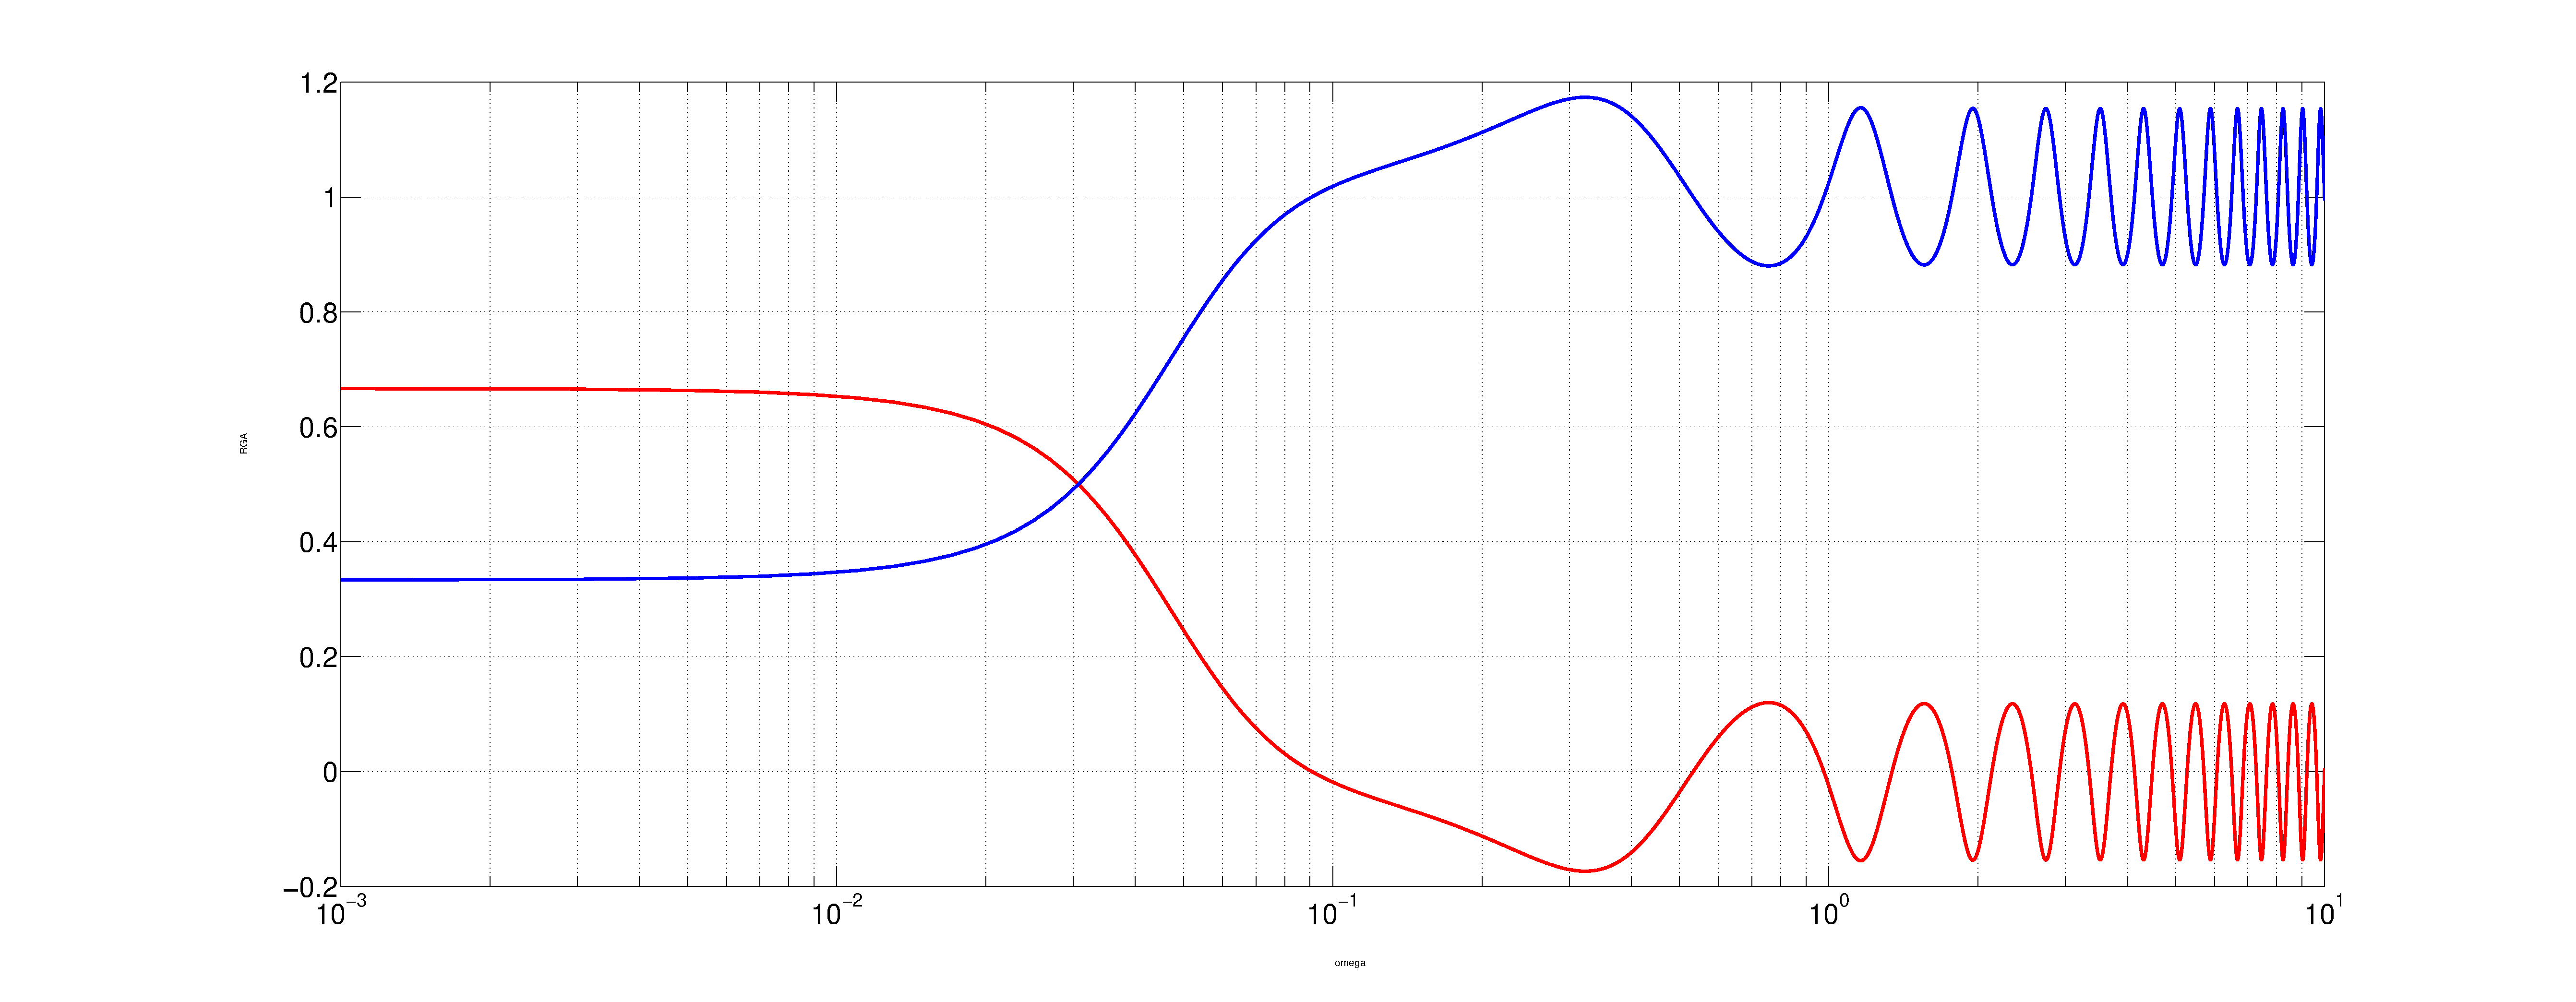
\includegraphics[scale=0.15]{fig/RG.eps}}
%\caption{RGA plot of $\vec{P}_n(s)$: diagonal elements of $\Lambda [\vec{P}_n(j\omega)]$ (blue, solid), off diagonal elements of $\Lambda [\vec{P}_n(j\omega)]$ (red, solid).}
%\label{fig:RGA}
%\end{figure}
%The most severe interaction occurs where $\Lambda_{qp}=0.5$ for $q=1,2$ and $p=1,2$. This can be seen in Fig. \ref{fig:RGA} as the intersecting point of $\Lambda [\vec{P}_n(j\omega)]$, which occurs at a frequency of approximately  0.0307 rad/min.
%Consider the case when $s=0$ (steady state response to a step input). The RGA matrix can be determined to be the following: 
%\begin{equation}
%\Lambda[\vec{P}_n(s)]\Big|_{s=0}=
%\begin{bmatrix}
%0.3333 & 0.6667 \\ 0.6667 & 0.3333
%\end{bmatrix}
%\end{equation}
%Since $0< \Lambda_{qp} < 1$ for $p,q=1,2$, interactions do exist, and the system is coupled. The permuted identity matrix can also be computed as follows:
%\begin{equation}
%\lim_{k \to \infty} \Lambda^k[\vec{P}_n(s)]\Big|_{s=0} = \begin{bmatrix}
%0.5 & 0.5\\0.5 & 0.5
%\end{bmatrix}
%\end{equation}
%which confirms that the plant process is not diagonally dominant at steady state. 
The performance and uncertainty filters chosen for this example will be identical to those in \cite{GKL10b},
\begin{equation}
W_{1_{q}}=0.5 \qquad W_{2_{q}}=0.5\left(\frac{2s+1}{s+1}\right) \qquad  q=1,2
\end{equation}
The desired diagonal open-loop transfer function $\vec{L}_D(s)$ will be chosen as simple integrators with time constants equal to 7 minutes (i.e, $\vec{L}_D(s)=diag\left(\frac{1}{7s}\right)$). For simplicity, a PI controller will be designed for this process. Since $\beta_{11}=\beta_{12}=\beta_{21}=\beta_{22}=2$, there will be a total of $m=16$ possible cases to consider in the design process. The optimization problem in (\ref{eq:long_con}) can now be solved by repeating the stability constraints for each combination of the uncertainties in (\ref{eq:mimo_un}). The frequency grid will be chosen to be between $10^{-2}$ and $10^{1}$ rad/min with $N=150$ equally spaced points. The PI MIMO controller obtained from the optimization problem is as follows:
\begin{equation}
\renewcommand{\arraystretch}{2.2}
\vec{C}(s)=
\begin{bmatrix}
\dfrac{0.06234s + 0.001464}{s} & \dfrac{-0.04803s - 0.005408}{s} \\
\dfrac{0.1585s + 0.0168}{s} & \dfrac{0.3113s + 0.005995}{s}
\end{bmatrix}
\end{equation}
Fig. \ref{fig:mimo1} displays the closed-loop MIMO response to a step input. Notice that with this controller, the MIMO process achieves robust performance while simultaneously decoupling the system. The Gershgorin bands are depicted in Fig. \ref{fig:mimo2} for the system possessing the largest delay time uncertainty ($\tau_{11}=9$, $\tau_{12}=13$, $\tau_{21}=15$, $\tau_{22}=11$). The red and blue bands possess a radius of $|r_{q}(j\omega_k)|$ for $q=1,2$ and $k=1,\ldots,N$. 
\begin{figure}[H]
\centering
\psfrag{tit1}{\hspace{-0.45cm} \scriptsize From $x_1$}
\psfrag{tit2}{\hspace{-0.45cm} \scriptsize From $x_2$}
\psfrag{tit3}{\hspace{-0.45cm} \scriptsize From $x_1$}
\psfrag{tit4}{\hspace{-0.45cm} \scriptsize From $x_2$}
\psfrag{im1}{\hspace{-0.3cm} \raisebox{0.1cm}{\scriptsize To $y_1$}}
\psfrag{im2}{\hspace{-0.3cm} \raisebox{0.1cm}{\scriptsize To $y_1$}}
\psfrag{im3}{\hspace{-0.3cm} \raisebox{0.1cm}{\scriptsize To $y_2$}}
\psfrag{im4}{\hspace{-0.3cm} \raisebox{0.1cm}{\scriptsize To $y_2$}}
\psfrag{re}{\hspace{-0.7cm} \raisebox{-0.05cm}{\scriptsize Time (minutes)}}
\centerline{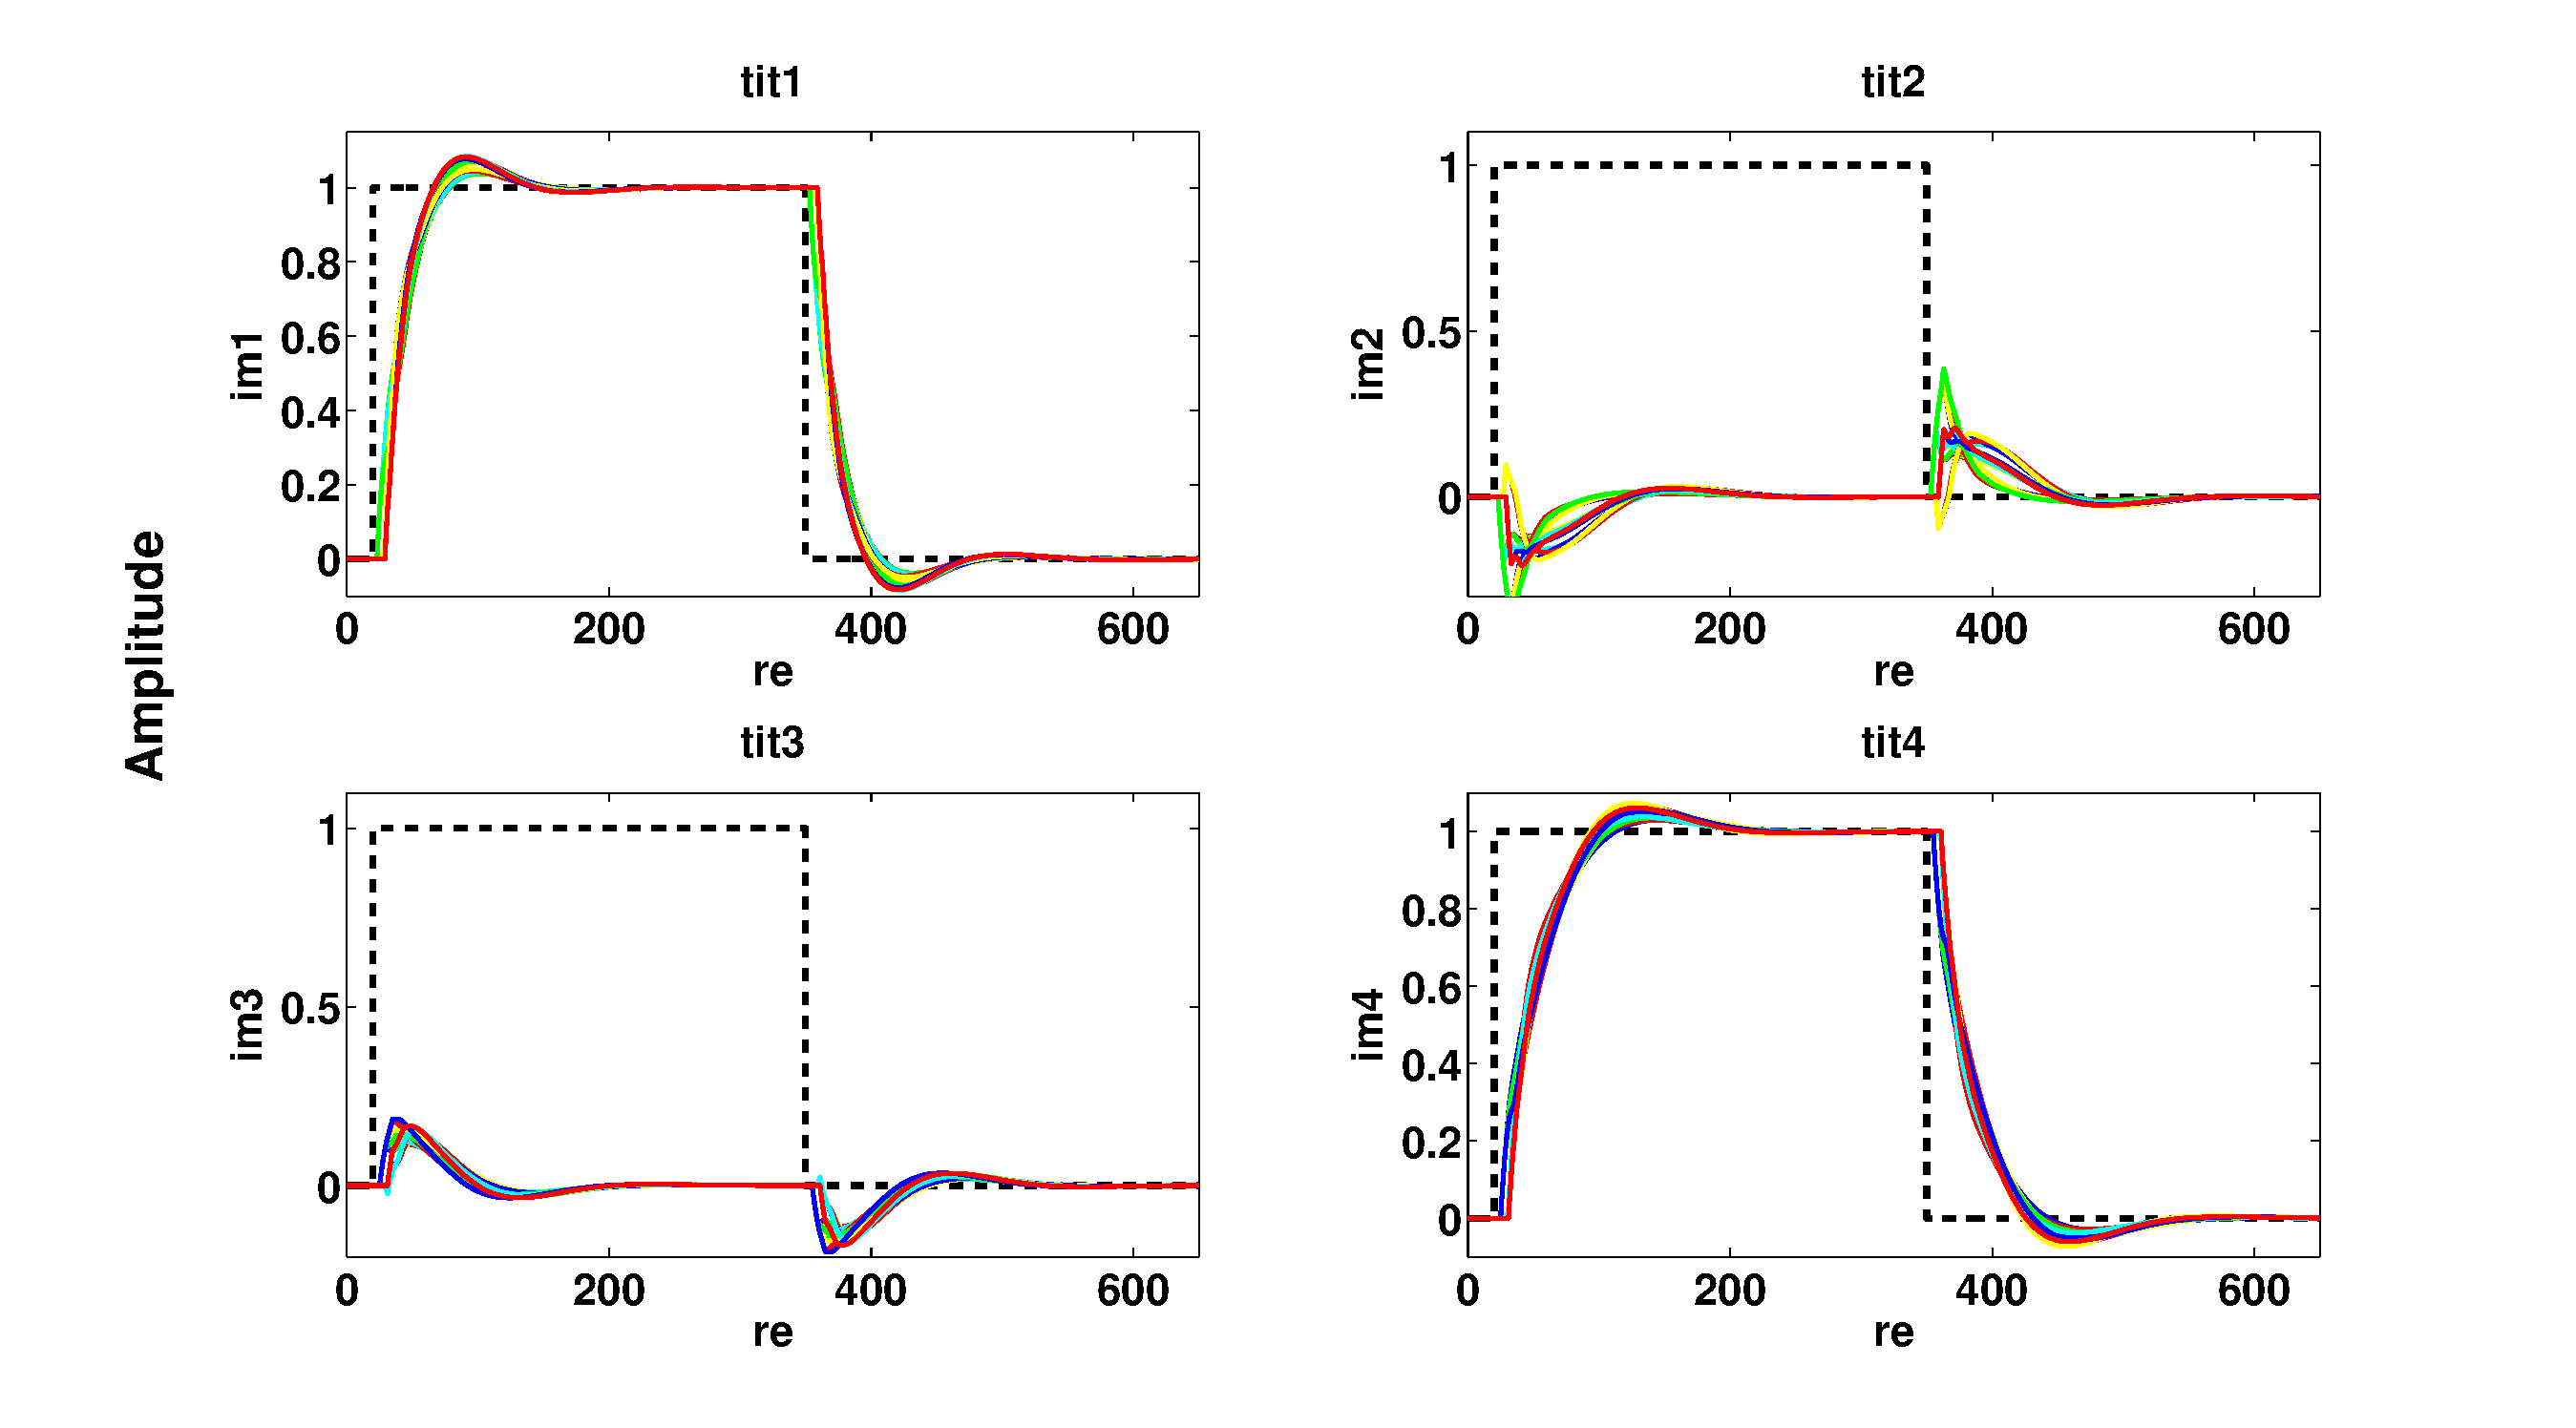
\includegraphics[width=13cm,height=6.5cm]{fig/test.eps}}
\caption{MIMO response to a unit step input: reference signal (black,dash), the remaining $\Omega=16$ closed-loop responses are for all possible combinations of the time delay parameters in (\ref{eq:mimo_un}).}
\label{fig:mimo1}
\end{figure}
\begin{figure}[H]
\vspace{-0.7cm}
\centering
\psfrag{R}{\hspace{-0.5cm}$\Re_e \{Z(j\omega) \}$}
\psfrag{Y}{\hspace{-0.7cm}$\Im_m \{Z(j\omega) \}$}
\centerline{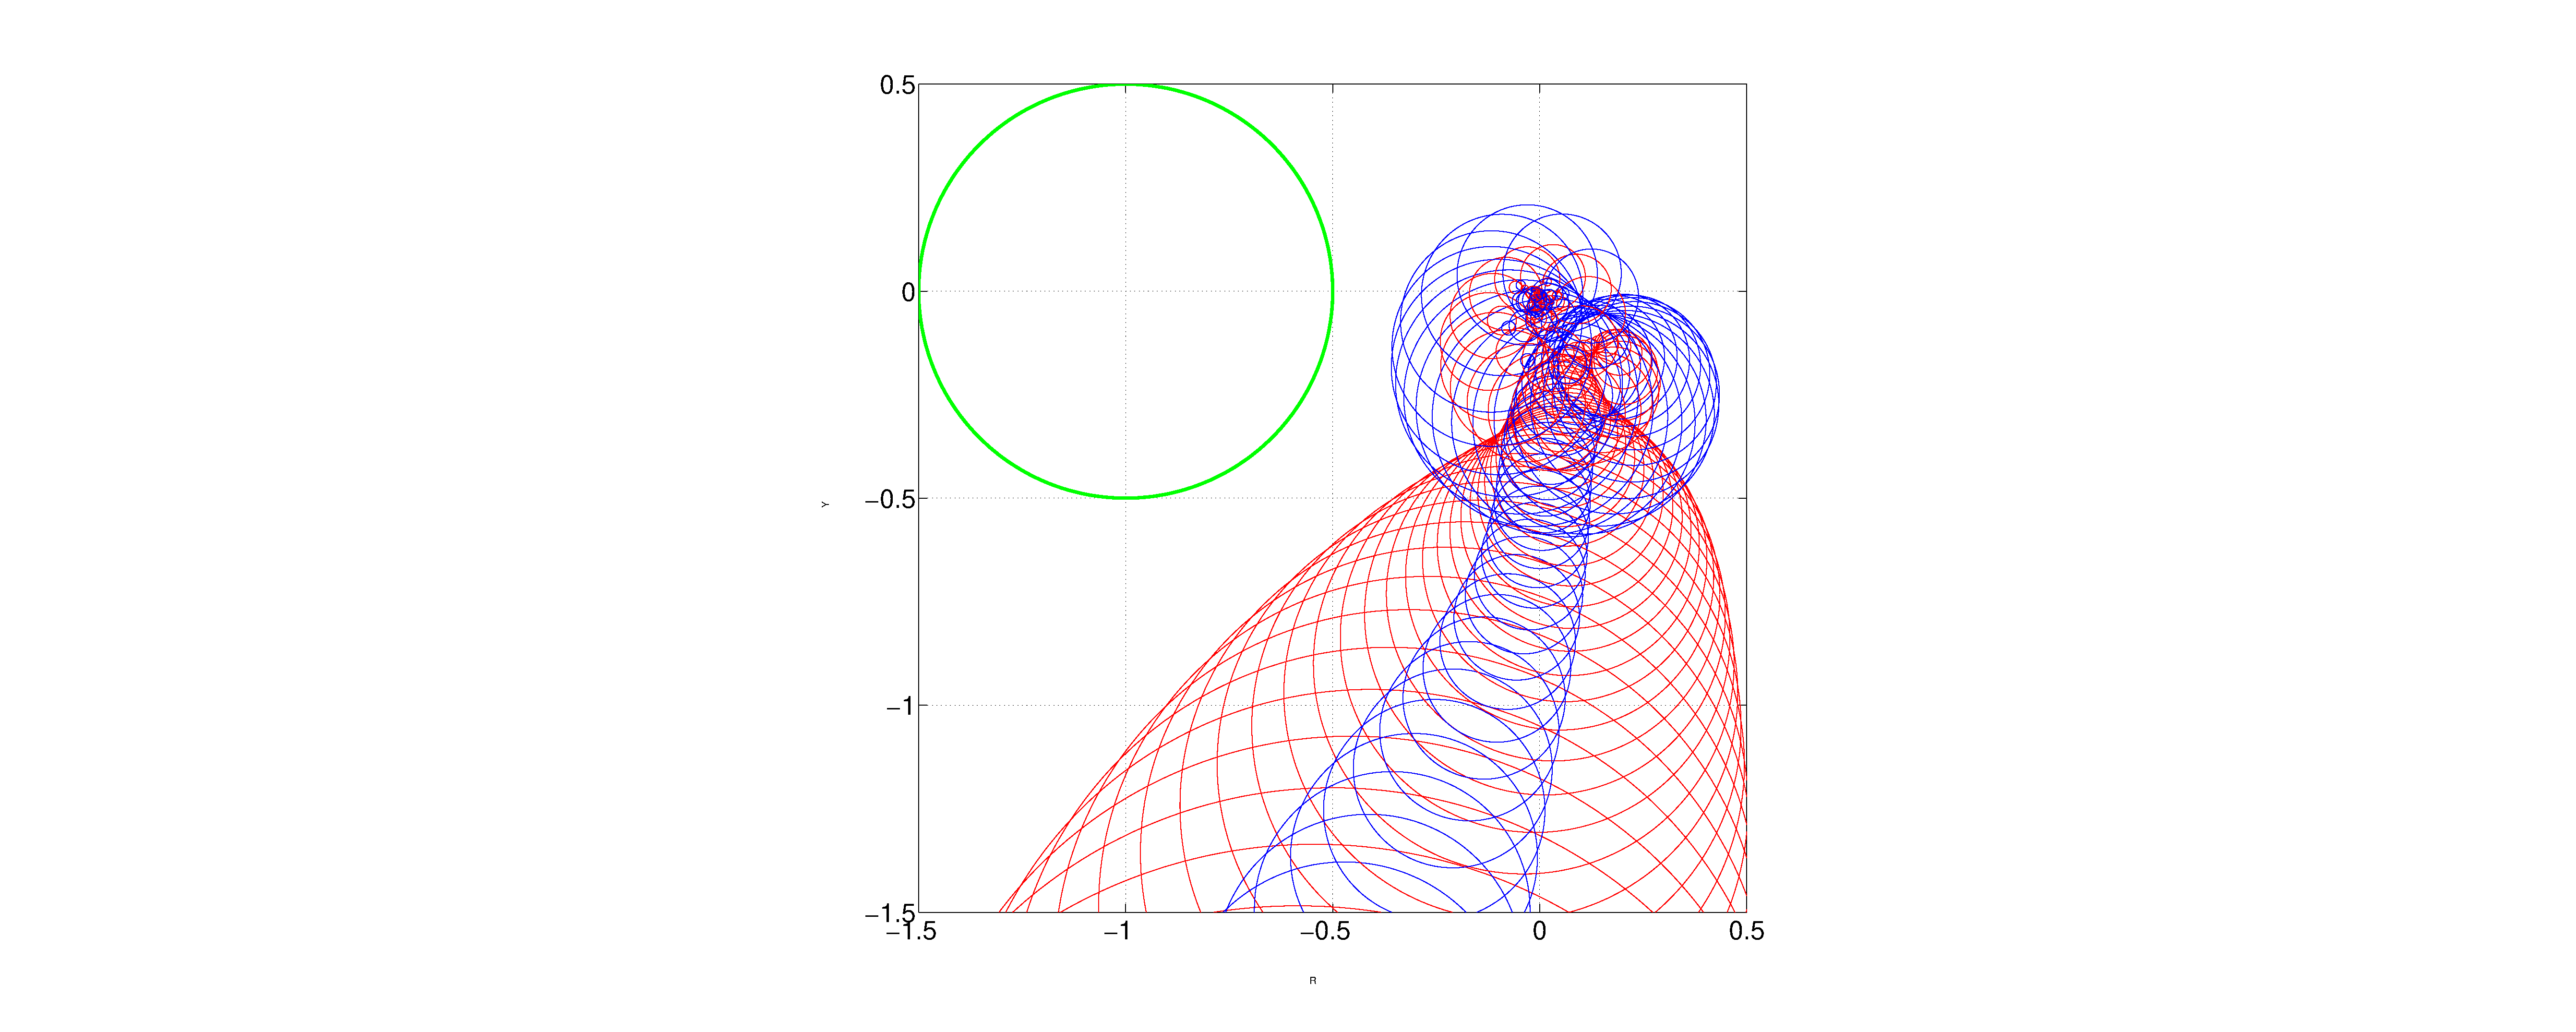
\includegraphics[scale=0.18]{fig/gersh.eps}}
\caption{Gershgorin bands for $L_{qq}$ with the largest time delay combination in (\ref{eq:mimo_un}): performance filter with $|W_{1_{q}}|=0.5$ (green circle), Gershgorin bands corresponding to $q=1$ (blue circles), Gershgorin bands corresponding to $q=2$ (red circles). Note that $Z(j\omega)$ is simply the complex number representation of each circle in the plot.}
\label{fig:mimo2}
\end{figure}
Notice how the Gershgorin bands never intersect with the performance circle centered at $(-1+j0)$. This proves that the MIMO system is stable, robust, and satisfies the optimization criterion in (\ref{eq:long_con}).  
\section{Extension to Unstable SISO Systems}
\label{sec:4}
The SP in the scheme shown in Fig. \ref{fig:dtc} cannot be used for unstable plants since the controller will contain zeros in right-hand side of the s-plan which cancel the unstable poles in the plant and leads to instability. 
To avoid this unstable zero-pole cancellation, the control structure shown in Fig.\ref{fig:dtc} should be changed. 
Several alternatives are available in literature to cope with unstable processes with dead-time (see, for example, \cite{Dep85,MA98,LCGZ05,NC07,NC09}).  

Consider, for instance, the SP with modified dead-time free model depicted in Fig.~\ref{fig:dtc_modified} which is discussed in \cite{NC07}. 
\begin{figure}
\centering
\psfrag{c}[cc][cc]{$C(s)$}
\psfrag{p}[cc][cc]{$P(s)$}
\psfrag{m}[cc][cc]{$G_m(s)-P_n(s)$}
\psfrag{y}[cc][cc]{$y$}
\psfrag{u}[cc][cc]{$u$}
\psfrag{r}[cc][cc]{$r$}
\centerline{{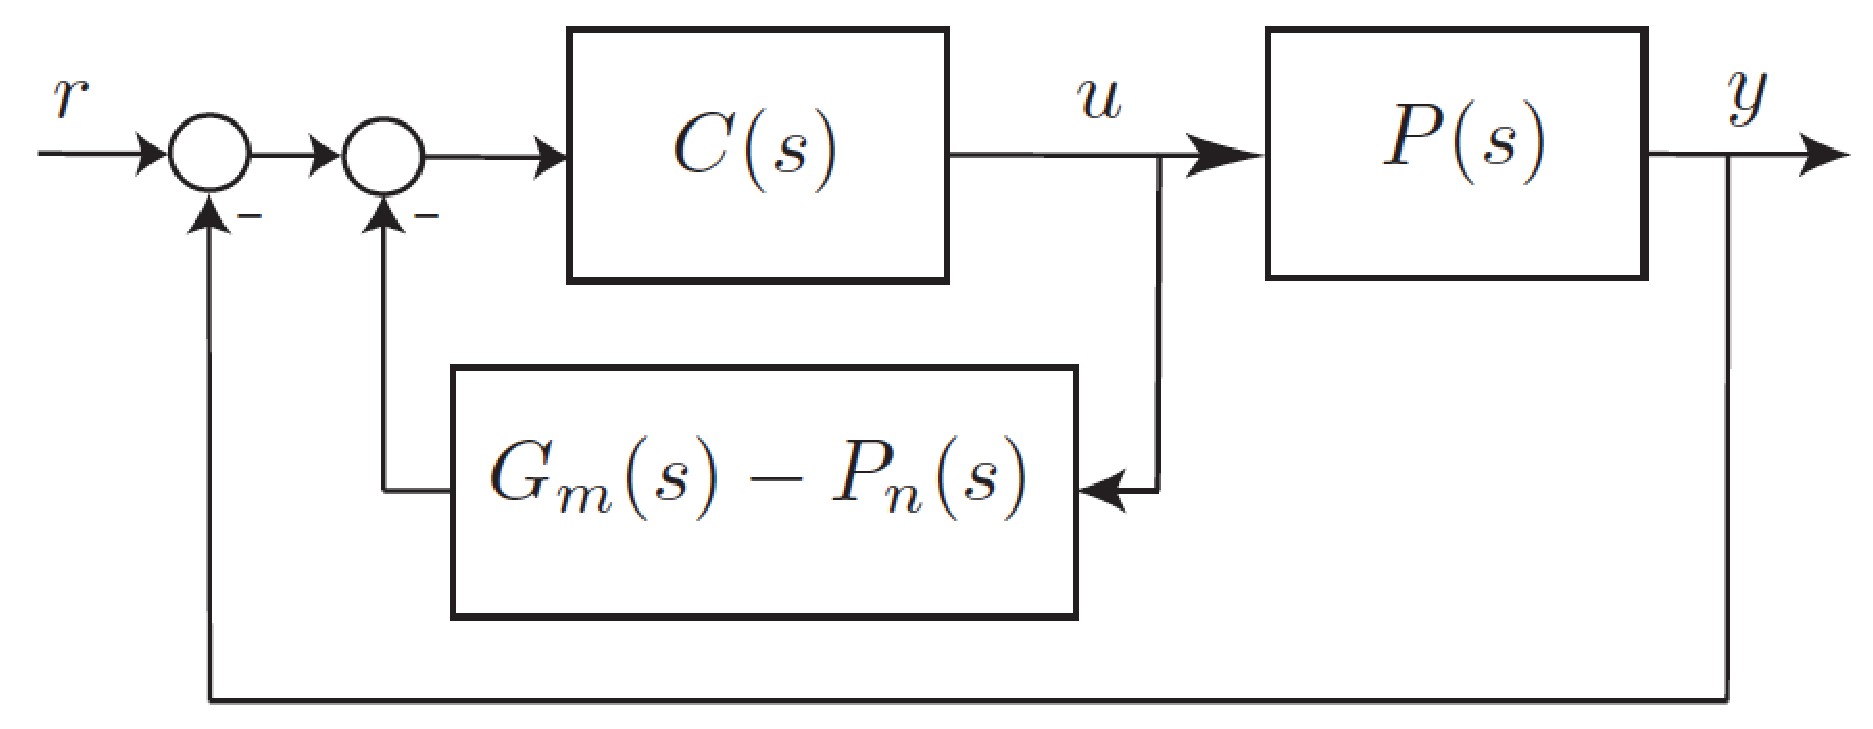
\includegraphics[scale=.26]{fig/uns.eps}}}
\caption{Smith Predictor with modified dead-time free model}
\label{fig:dtc_modified}
\end{figure}%
In this case, the dead-time free model is defined as $G_m=\frac{N_m}{D_n}$ and $H=G_m-P_0=(N_m -N_ne^{-\tau s})\frac{1}{D_n}$. Therefore, $N_m$ must be tuned such that the zeros of $N_m -N_ne^{-\tau s}$ cancel the unstable poles in $D_n$. Once $N_m$ has been properly designed, the primary controller can be obtained by solving the optimization problem in (\ref{eq:min_hinf}) redefining $H=G_m-P_0$ and
$L_i(\rho)=(G_m-P_0+P_i)C(\rho)$. Here, care should be taken in the choice of $L_d$. As it has been shown, the $wno$ of $1+L_i$ equals the $wno$ of $1+L_d$. Therefore, $L_d$ should be chosen such that the number of encirclement of the critical point $(-1+0j)$ by its Nyquist plot is equal to the number of unstable poles in $P_i$.

\subparagraph{Example 3}
Consider the model studied in \cite{MZ00} given by:
\begin{equation}
P(s)=\frac{k}{s-a}[1+\Delta(s)W_2(s)]e^{-\tau s}
\end{equation}  
where $k=1$, $a=1$, $\tau=\tau_n \pm 0.02$ and $\tau_n=0.2$. The interval of variation of $\tau$ is gridded using $q=3$ equally spaced points. A finer grid just increases the number of constraints and for this example does not change significantly the final controller.
The performance and uncertainty filters are respectively chosen as:
\begin{equation}
W_1(s)=2\left(\frac{s+1}{10s+1}\right) \quad \mbox{and} \quad  W_2(s)=0.2\left(\frac{s+1.1}{s+1}\right)
\end{equation}
%The objective is to minimize $\gamma$ such that the robust performance condition $\|  |W_1S_i|+|W_2T_i|	  \|_{\infty}<\gamma$ holds for $i=1,2,3$. 

Here, we use the SP with modified dead-time free model (Fig. \ref{fig:dtc_modified}) due to its simplicity. The dead-time free model $G_m(s)$ is chosen as
\begin{equation}
G_m(s)=\frac{T_ms+1}{s-1}.
\end{equation}
$T_m$ is computed in order to obtain $H(s)=G_m(s)-P_0(s)$ without a pole in $s=1$.
Since 
\begin{equation}
H(s)=\frac{1}{s-1}[T_ms+1-e^{-0.2s}],
\end{equation}
if $T_m=e^{-0.2}-1$, then $s=1$ is a zero of $H(s)$.

A PI as the primary controller is designed. The first step is to choose the transfer function $L_d(s)$, which must encircle the critical point in the Nyquist diagram once and must contain one integrator. Therefore, it is chosen as
\begin{equation}
L_d(s)=10\frac{s+1}{s(s-1)}.
\end{equation}
Optimization problem (\ref{eq:min_hinf}) is solved considering $N=100$ equally spaced frequency points between $\omega=10^{-3}$rad/s and $\omega=10^{3}$rad/s and the following controller is obtained:
\begin{equation}
C_{0}(s)=(3.582 s + 0.5838)/s
\end{equation}  
which yields $\gamma= 0.6854$. This result can be further improved by using a new $L_d(s)$ based on $C_0(s)$ in the optimization problem. With this new $L_d(s)=G_m(s)C_0(s)$ the optimal primary controller is: 
\begin{equation}
C(s)=(2.994 s + 0.4612)/s
\end{equation}  
and $\gamma=0.6074$. Figure \ref{fig:example3} depicts the function 
$$\Gamma_i(j\omega)=|W_1(j\omega)S_i(j\omega)|+|W_2(j\omega)T_i(j\omega)|$$
where $S_i$ and $T_i$ are respectively given by (\ref{eq:sensitivity}) and (\ref{eq:sensitivity_comple}) with $H=G_m-P_0$ and $P_i$ is obtained by gridding of $\tau$. Note that the maximum value of the function is $0.6072$, which occurs when $\tau=\tau_n+0.02=0.22$, is close to the bound $\gamma$. It is worth to point out that, although the conditions given in Theorem \ref{th:siso} are only sufficient to guarantee $\| \Gamma_i \|_{\infty}<\gamma$, with a proper choice of $L_d$ it is possible to obtain 
a solution with very low conservatism. Furthermore, the resulting controller is a standard PI 
which can be implemented in a straightforward manner and has great practical significance.
\begin{figure}[!h]
\centering
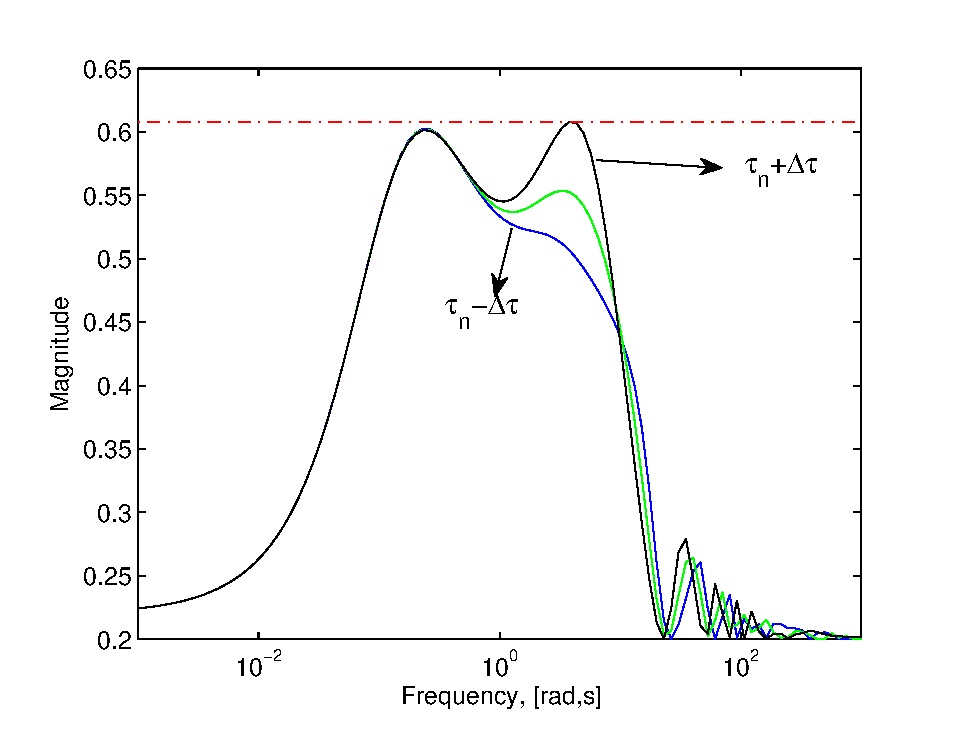
\includegraphics[width=0.7\columnwidth]{fig/shaped_sensitivity}
\caption{Example 2: Blue solid line: $\Gamma$ for $\tau=0.18$; green solid line: $\Gamma$ for $\tau=0.2$;  black solid line: Blue solid line: $\Gamma$ for $\tau=0.22$; red dot-dashed line: $\gamma$.}
\label{fig:example3}
\end{figure}

%The equivalent controller $C_{eq}$ obtained in \cite{MZ00} can be written as
%\begin{equation}
%C_{eq}=\frac{K}{1-KF_{stab}}
%\end{equation}
%where the primary controller $K$ is:
%\begin{equation}
%K=\frac{4.6971s^2+5.6971s+1}{0.000016s^3+1.4414s^2+1.4792s+0.0379}
%\end{equation}
%and the predictor $F_{stab}$ is given by:
%\begin{equation} 
%F_{stab}=\frac{-10.75 s^2 - 0.245 s + 0.3298}{12.03 s^3 - 12.03 s^2 + s - 1
%}+\frac{(13.16 s^2 - 0.1316)e^{-0.2s}
%}{12.03 s^3 - 12.03 s^2 + s - 1}
%\end{equation}
%The $\Gamma_i(j\omega)$ function for this controller with $i=1,2,3$ is depicted on Fig. \ref{fig:unstable_compare}. 

For the same example, controller designed in \cite{MZ00} leads to  the optimal $\gamma = 0.9407$ which is 55\% higher than the value obtained with the proposed method. It should be mentioned that the true robust performance criterion in (\ref{eq:min_hinf}) is not minimized in \cite{MZ00}. Instead, the maximum singular value of $[W_1(j\omega)S(j\omega) \quad W_2(j\omega)T(j\omega)]$ for all $\omega$ is minimized by the $H_\infty$ control theory. 
 

%\begin{figure}[!h]
%\centering
%\includegraphics[width=\columnwidth]{pics/example2/gamma_compare}
%\caption{Example 2, controller from \cite{MZ00}:  Blue solid line: $\Gamma$ for $\tau=0.18$; green solid line: $\Gamma$ for $\tau=0.2$;  black solid line: Blue solid line: $\Gamma$ for $\tau=0.22$.}
%\label{fig:unstable_compare}
%\end{figure}
%

\section{Gain-scheduled Controller Design}
\label{sec:5}
Consider an uncertain plant $P(s,\theta)$ belonging to the set:
\begin{equation}
\mathsf{P}_\theta=\{G(s,\theta)e^{-\tau_i(\theta)s}, \; i=1,\dots, q \}
\end{equation}
where the dead-time free part of the model has unstructured multiplicative uncertainty and is described as:
\begin{equation}
G(s,\theta)=G_n(s,\theta)[1+\Delta(s) W_2(s)]
\end{equation}
and $\theta$ is a vector of scheduling parameters that belongs to a finite set $\Theta=\{\theta_1, \theta_2, \ldots, \theta_m   \}$ (corresponding e.g. to the different operating point parameters). It is assumed that the operating point does not frequently change (the stability and performance are achieved for the frozen scheduling parameter). The dead-time is also a function of the scheduling parameter and uncertain, so for a given value of $\theta$ it belongs to the set $\{ \tau_1(\theta), \tau_2(\theta), \ldots, \tau_q(\theta)    \}$. 

We will consider the SP shown in Fig. \ref{fig:dtc_lpv} where both, the nominal model $P_0(s,\theta)=G_n(s,\theta)e^{-\tau_n(\theta)s}$ and the primary controller $C(s,\theta)$ are functions of the scheduling parameter vector $\theta$. The goal is to compute a primary gain-scheduled controller for this scheme that meets the $H_\infty$ robust performance specification. 
\begin{figure}
\centering
\psfrag{rr}{\small $r$}
\psfrag{cc}{\small \hspace{-0.1cm}$C(s,\theta)$}
\psfrag{uu}{\small $u$}
\psfrag{pp}{\small \hspace{-0.15cm}$P(s,\theta)$}
\psfrag{gn}{\small \hspace{-0.2cm}$G_n(s,\theta)$}
\psfrag{ex}{\small \hspace{-0.2cm}$e^{-\tau_n(\theta) s}$}
\psfrag{yp}{\small $y_p$}
\psfrag{yy}{\small $y$}
\psfrag{pl}{\small $+$}
\psfrag{mi}{\small $-$}
\psfrag{dis}{\small $d$}
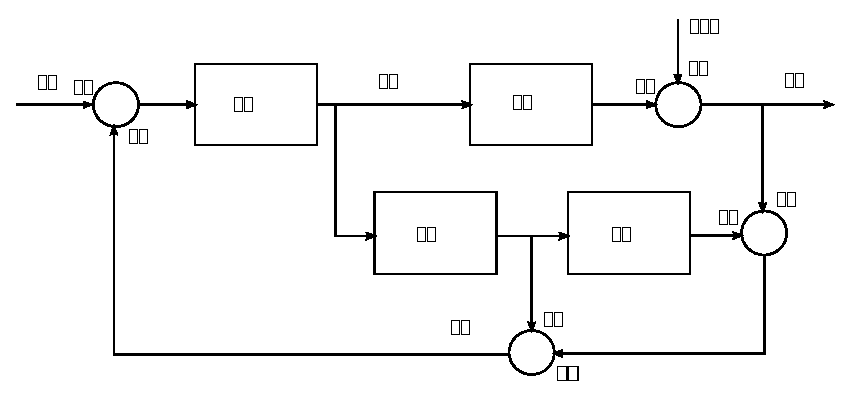
\includegraphics[scale=0.7]{fig/SISO_block.eps}
\caption{Gain-Scheduled Smith Predictor}
\label{fig:dtc_lpv}
\end{figure}%
 
The primary controller ${C}(s,\theta)$ is linearly parametrized by:
$
C(s,\theta)=\rho^T(\theta) \phi(s)
$,
where the basis function vector $\phi(s)$ is defined as in section (\ref{sec:siso_cls}) and $\rho^T(\theta)$
is given by
\begin{equation}	
 \rho^T(\theta)=[\rho_{1}(\theta),\rho_{2}(\theta), \ldots, \rho_{n}(\theta)]
\end{equation}
Every gain is a polynomial function of order $\delta$  of the scheduling parameters and is defined as
\begin{equation}
\rho_{i}(\theta)=(\nu_{i, \delta})^T\theta^{\delta}+\ldots+(\nu_{i, 1})^T\theta+ \nu_{i, 0}
\end{equation}
and $\theta^{k}$ denotes element-by-element power of $k$ of vector $\theta$.
In Fig. (\ref{fig:dtc_lpv}), the transfer function from the output disturbance $d$ to $y$ is the sensitivity function $S_i(s,\theta)$, while the transfer function from $r$ to $y$ is the complementary function $T_i(s,\theta)$:
\begin{align}
S_i(s,\theta)&=\frac{1+C(s,\theta)H(s,\theta)}{1+C(s,\theta)(H(s,\theta)+P_i(s,\theta)) } \\ \nonumber
T_i(s,\theta)&=\frac{C(s,\theta)P_i(s,\theta)}{1+C(s,\theta)(H(s,\theta)+P_i(s,\theta)) }, \; \forall \theta \in \Theta
\end{align}
where $H(s,\theta)=G_n(s,\theta)-P_0(s,\theta)$. The primary controller is obtained from the following optimization problem:
\begin{align}\label{eq:min_hinf_lpv}
&\qquad \min_{\rho} \gamma \nonumber \\\mbox{Subject to:} &\\ \nonumber
& \|  |W_1S_i(s,\theta)| + |W_2T_i(s,\theta)| \|_{\infty}<\gamma\\ 
& \mbox{for } i=1,\dots,q,  \quad \forall \theta \in \Theta \nonumber
\end{align}

%
%As an LPV model is available, there will be an infinity
%number of models corresponding to different values of the
%scheduling parameters. 
%This problem can be solved by gridding
%$\theta$ leading to $m$ different LTI models. Considering the multimodel uncertainty,
%the procedure should be repeated for each one of the $q$ uncertain models. 

Optimization problem (\ref{eq:min_hinf_lpv}) is again solved using an iterative bisection algorithm as previously presented. At each iteration, a feasibility problem is solved with the following convex constraints:
\begin{eqnarray} \label{eq:cond_lpv}
\Big [ |W_{1}(j\omega_k)[1+C(j\omega_k,\theta_l)H(j\omega_k,\theta_l)|+|W_{2}(j\omega_k)C(j\omega_k,\theta_l)P(j\omega_k,\theta_l) | \Big ] \nonumber\\ \times |1+L_{d}(j\omega_k)|-
Re\{[1+L^{\ast}_{d}(j\omega_k)][1+L_i(j\omega_k,\theta_l)]\}<0 \nonumber\\ \mbox{for } k=1,\dots,N,\quad  i=1,\ldots,q, \quad l=1,\ldots,m  
\end{eqnarray}
%where $\theta_l$ is a vector with particular values of the scheduling
%parameters $\theta$ obtained from the gridding. 

%It should be noted that since the design is performed in the frequency domain, the designed controller guarantees the closed-loop stability and performance for frozen scheduling parameters.

\subparagraph{Example 4}
The design method is applied on a simulated system having a resonance
whose frequency changes as a function of a scheduling
parameter $\theta$. Consider the following plant model
\begin{equation}
P(s,\theta)=G(s,\theta)e^{-\tau s}
\end{equation}
where $G(s,\theta)=G_n(s,\theta)[1+\Delta(s)W_2(s)]$ and
\begin{eqnarray}
G_n(s,\theta)&=&\frac{(2+0.2\theta)^2 }{s^2+0.2(2+0.2\theta)s+(2+0.2\theta)^2} \\
W_2(s)&=&0.8\frac{1.1337s^2+6.8857s + 9}{(s+1)(s+10)}
\end{eqnarray}
and $\theta \in [-1, -0.5, 0, 0.5, 1]$.
%This model could represent the dynamics of a mechatronic
%system, where the frequency of the resonance is a function of
%the moving mass. 
Consider also that the dead-time is within the interval $\tau \in [2.7, 3.0, 3.3]$ but its exact value is unknown in runtime. 
The objective is to design a primary gain-scheduling PID controller for the Smith Predictor structure  considering the performance filter 
$
 W_1(s)=\frac{2}{(20s+1)^2}
$.
 The parameters $\rho$ of the primary controller will be affine functions of the scheduling parameter $\theta$. The filter of the derivative
action is chosen to have a time constant of $T_f=0.01$s.
%The range of the scheduling parameter $\theta$ is gridded using $m=5$ points. The uncertainty interval of the dead-time is gridded using $q=3$ points.   

Finally, optimization problem (\ref{eq:min_hinf_lpv}) is solved considering $L_d=1/s$ and $N=100$ equally spaced frequency points between $10^{-2}$ and $10^2$ rad/s. 
The resulting gain-scheduled controller is given by:
$K_p(\theta)=   -0.0168 \theta +     0.2152$, $K_i(\theta)=  0.0144\theta +   2.4736$, 
$K_d(\theta)=-0.1224 \theta+   0.6424$.

This controller leads to:
\begin{align}
&\|  |W_1S_i(s,\theta_l)| + |W_2T_i(s,\theta_l)| \|_{\infty}<\gamma=0.8928\\ \nonumber
&l=1,\ldots,5, \quad i=1,2,3
\end{align}
The gain-scheduled controller is evaluated considering $\theta=-1,0,1$ and $\tau=3.3$s. The performance is compared to a fixed-gain PID designed for the nominal case ($\theta=0$ and $\tau= 3$s). Figure \ref{fig:example2} shows the step response of the gain-scheduled controller in all conditions (blue, red and green solid lines) compared with the fixed PID controller (black dashed line, highly oscillating). 
\begin{figure}[H]
\centering
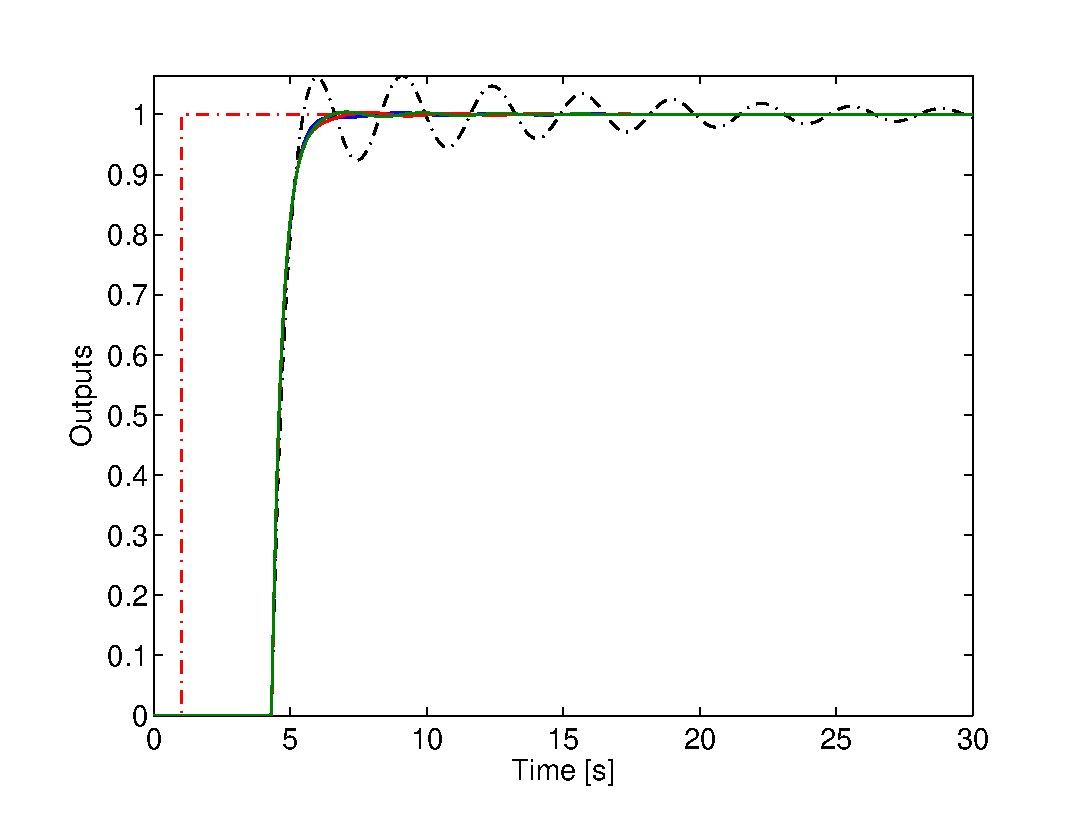
\includegraphics[scale=0.4]{fig/exampleLPV_min_gamma}
\caption{Example 3: Blue, red and green solid line: gain-scheduled PID Smith Predictor and $G_2$ using  $\theta_1=-1$, $\theta_3=0$ and $\theta_5=1$ respectively;  black dashed line: fixed PID Smith Predictor using $\theta=-1$.}
\label{fig:example2}
\end{figure}%


\section{Conclusions}
This paper presents a new method to design a robust Smith Predictor for uncertain SISO and MIMO time-delay systems using convex optimization techniques. The proposed approached allows one to design PI/PID as well as higher order primary controllers in the Smith Predictor structure which provide robust $H_{\infty}$ performance for systems with uncertain dead-time and multiplicative or multimodel uncertainty in the dead-time free model of the system. The method is based on a convex approximation of the $H_\infty$ robust performance criterion in the Nyquist diagram. This approximation relies on the choice of a desired open-loop transfer function $L_d$ for the dead-time free model of the plant. For the SISO case, a bisection algorithm was implemented to solve the convex constrained problem. For the MIMO case, a controller was designed such that the system became decoupled and simultaneously optimized the single-loop performances of the SISO subsystems.

%The controller design examples shown for both MIMO and SISO cases considered a finite amount of discrete values to represent the uncertainties in the time delays. However, the proposed optimization methods can be applied for a system(s) with $\alpha$ number of uncertainties within a specified range, where $\{\exists\alpha \in \mathbb{Z}^+ | \; 0<\alpha<\infty \} $.

%For SISO systems, the number of combinations to consider in the controller design will simply be the number of elements $M$ in the uncertain set. However, for MIMO systems, the number of combinations will be $M^{n_o n_i}$ (assuming the same number of uncertainties for each time delay). For example, a SISO system containing a range of time delays with three uncertainties will have to compute a controller for $M=3$ combinations. On the other hand, a $3 \times 3$ MIMO system with the same number of uncertainties will have to consider $M^{n_o n_i}=3^9=19,683$ combinations. Thus the controller design for MIMO systems will be computationally expensive for systems with a large amount of inputs and outputs.
\begin{thebibliography}{99.}%
% and use \bibitem to create references.
%
% Use the following syntax and markup for your references if
% the subject of your book is from the field
% "Mathematics, Physics, Statistics, Computer Science"
%
% Contribution
\bibitem{Bro79} C. B. Brosilow. The structure and design of Smith
predictors from the viewpoint of inferential control.
In Proceedings of Joint American Control Conference,
Denver, Colorado, 1979.
%
\bibitem{Dep85} A. M. De Paor. A modified Smith predictor and controlled
for unstable processes with time delay. International
Journal of Control, 41(4):1025--1036, 1985.
%
\bibitem{DFT92} C. J. Doyle, B. A. Francis, and A. R. Tannenbaum.
Feedback Control Theory. Mc Millan, New York, 1992.
%
\bibitem{GKL10a} G. Galdos, A. Karimi, and R. Longchamp. Robust controller
design by convex optimization based on finite
frequency samples of spectral models. In 49th IEEE
Conference on Decision and Control, Atlanta, USA,
2010a.
%
\bibitem{GKL10b} G. Galdos, A. Karimi, and R. Longchamp. $H_{\infty}$ controller
design for spectral MIMO models by convex optimization.
Journal of Process Control, 20(10):1175--1182,
2010b.
%
\bibitem{Hag92} T. Hagglund. A predictive PI controller for processes with
long dead times. IEEE Control Systems Magazine, 12
(1):57--60, 1992.
%
\bibitem{HWC95} C. C. Hang, Q. Wang, and L. S. Cao. Self-tuning Smith
predictors for processes with long dead time. International
journal of adaptive control and signal processing,
9(3):255--270, 1995.
%
\bibitem{KG10} A. Karimi and G. Galdos. Fixed-order $H_{\infty}$ controller design
for nonparametric models by convex optimization.
Automatica, 46(8):1388--1394, 2010.
%
\bibitem{Kay01} I. Kaya. Tuning Smith predictors using simple formulas
derived from optimal responses. Industrial and engineering
chemistry research, 40(12):2654--2659, 2001.
%
\bibitem{LLSL99} D. Lee, M. Lee, S. Sung, and I. Lee. Robust PID tuning
for Smith predictor in the presence of model uncertainty.
Journal of Process Control, 9(1):79--85, 1999.
%
\bibitem{LCGZ05} T. Liu, Y. Z. Cai, D. Y. Gu, and W. D. Zhang. New
modified Smith predictor scheme for integrating and
unstable processes with time delay. IEE Proceedings-
Control Theory and Applications, 152(2):238--246, 2005.
%
\bibitem{MA98} S. Majhi and D. P. Atherton. A new Smith predictor and
controller for unstable and integrating processes with
time delay. In Proceedings of the 37th IEEE Conference
on Decision and Control, pages 1341--1345, 1998.
%
\bibitem{MZ00} G. Meinsma and H. Zwart. On $H_\infty$ control for dead-time
systems. IEEE Transactions on Automatic Control, 45
(2):272--285, 2000.
%
\bibitem{Mir03} L. Mirkin. On the extraction of dead-time controllers
and estimators from delay-free parametrizations. IEEE
Transactions on Automatic Control, 48(4):543--553,
2003.
%
\bibitem{NC00} J. E. Normey-Rico and E. F. Camacho. Multivariable generalised predictive controller based on the Smith predictor. IEEE Proceedings in Control Theory Applications, Vol. 147, No. 5, 2000.
%
\bibitem{NC07} J. E. Normey-Rico and E. F. Camacho. Control of dead-time
processes. Springer Verlag, 2007.
%
\bibitem{NC09} J. E. Normey-Rico and E. F. Camacho. Unified approach
for robust dead-time compensator design. Journal of
Process Control, 19(1):38--47, 2009.
%
\bibitem{Pal80} Z. J. Palmor. Stability properties of Smith dead-time compensator
controllers. International Journal of Control,
32:937--949, 1980.
%
\bibitem{Pal96} Z. J. Palmor. Time-delay compensation Smith predictor
and its modifications. In W. Levine, editor, The Control
Handbook. CRC Press, Boca Raton, FL, 1996.
%
\bibitem{PB94} Z. J. Palmor and M. Blau. An auto-tuner for Smith dead
time compensator. International Journal of Control, 60
(1):117--135, 1994.
%
\bibitem{SBP09} R. S. Sanchez-Pena, Y. Bolea and V. Puig. MIMO Smith predictor: Global and structured robust performance analysis. Journal of Process Control 19:163-177, 2009.
%
\bibitem{SS93} C. Santacesaria and R. Scattolini. Easy tuning of Smith
predictor in presence of delay uncertainty. Automatica,
29(6):1595--1597, 1993.
%
\bibitem{Sko} S. Skogestad and I. Postlethwaite. Multivariable Feedback Control; Analysis and Design. John Wiley and Sons, England, 1996.
%
\bibitem{Smi57} O. J. M. Smith. Closer control of loops with dead time.
Chemical Engineering Progress, 53(5):217--219, 1957.
%
\bibitem{ZL06} W. Zhang and C. Lin. Multivariable Smith Predictors Design for Nonsquare Plants. IEEE Transactions on Control Systems Technology,
Vol. 14, No. 6, 2006.
%
\bibitem{Zho03a} Q. C. Zhong. On standard $H_\infty$ control of processes with a single delay. IEEE Transactions on Automatic Control,
48(6):1097--1103, 2003.
%
\bibitem{ZhoDoy} K. Zhou and J. Doyle. Essentials of Robust Control. Prentice-Hall, Upper Saddle River, New Jersey, USA, 1998.
%
\bigskip
\end{thebibliography}


\end{document}



